\documentclass[12pt,a4paper]{report}
% all configuration for the document

\usepackage[utf8]{inputenc}
\usepackage{amsmath}
\usepackage{amsfonts}
\usepackage{amssymb}
\usepackage{graphicx}
\usepackage{hyperref}
%\usepackage[margin=2.5cm]{geometry}
\usepackage{url}
\usepackage{pgffor}
\usepackage{enumitem}
%\usepackage{palatino}
\usepackage{siunitx}
\usepackage{array,booktabs}
\usepackage{subcaption}
\usepackage{cite}
\usepackage[table]{xcolor}

%%% for the draft watermark
%\usepackage{draftwatermark}
%\SetWatermarkText{DRAFT}
%\SetWatermarkScale{1}

%\usepackage[bindingoffset=0.5cm,margin=2cm]{geometry}
%\usepackage[font=small,labelfont=bf,skip=0pt]{caption}

\graphicspath{{G:/Projects/R2E/CHARM/Simulations/prelim_10nov/plots/}}

\newcommand*{\DirectoryDose}{./no_norm/dose_test_area_}
\newcommand*{\DirectoryHEH}{./no_norm/heh_test_area_}
\newcommand*{\DirectoryN}{./no_norm/n1meveq_test_area_}

\newcommand*{\Config}
{
cpOOOO_nn,
cpCIIC_nn,
alOOOO_nn,
alCIIC_nn,
alhOOOO_nn,
alhCIIC_nn}

\newcolumntype{P}[1]{>{\centering\arraybackslash}p{#1}}

\begin{document}
\title{CHARM Facility Test Area Radiation Field}
\date{February 2015}
\author{Adam Thornton}
\maketitle

\begin{abstract}
Specification document summarising the radiation field of the CHARM facility test area. This will act as a guide to any potential users of the facility as to what they can expect in terms of radiation, given in the form of radiation spectra information and fluence for each test position, along with general radiation maps for the test area and Montrac test location. \\
\end{abstract}

\tableofcontents

\section{Introduction}
% background and context, can get this from thesis and safety document

The CERN High Energy Accelerator Mixed-field (\href{http://charm.web.cern.ch/CHARM/}{CHARM}) facility is situated in the Proton Synchrotron (PS) East Area hall at the Meyrin Site of CERN in Switzerland. A map in figure \ref{fig:meyrin_map} shows the location on the Meyrin site, and a 3D rendered image of the East Area hall is shown in figure \ref{fig:eastarea_hall_3d}. The aim of the CHARM facility is to have a flexible and dedicated place for the testing of electronics and systems in well characterised mixed-radiation fields, which can replicate a wide number of real radiation environments such as space, atmosphere, or accelerator complexes for example. To achieve this, the test area has been constructed with the sole purpose of flexibility in electronics testing. \\

Starting with the 24 GeV proton beam from the PS, the beam is directed along a number of beam-lines to various physics experiments. The CHARM facility is located at the end of the T8 beam-line in the PS East Area Hall. The T8 beam-line is shared with the IRRAD facility, located up-stream of CHARM. Once the beam passes through IRRAD, it enters the CHARM test area where it impinges on 1 of the 3 possible targets (and alternatively without target). Depending on the target selection, the radiation field can be varied inside the test area. Additionally, there are 4 movable shielding layers of iron and concrete inside the test area which can further alter the radiation field. Finally there are a number of dedicated test positions around the test area, which are selected based on the radiation field requirements of the user. \\
 
To understand the radiation field within the test area, dedicated FLUKA \cite{FLUKA1} \cite{FLUKA2} Monte Carlo calculations have been made for the various facility configurations and test positions. Using these results, one can describe the radiation spectra seen at each test position and calculate useful quantities related to electronics testing, such as the total ionising dose (TID) or 1 MeV equiverlent neutron fluence in Silicon for example. A detailed list of the available information is shown in chapter 3. These values can then be used to calculate failure rates and tolerances of test equipment to be installed and used in environments where radiation is present. \\

\begin{figure}[!ht]
	\centering
	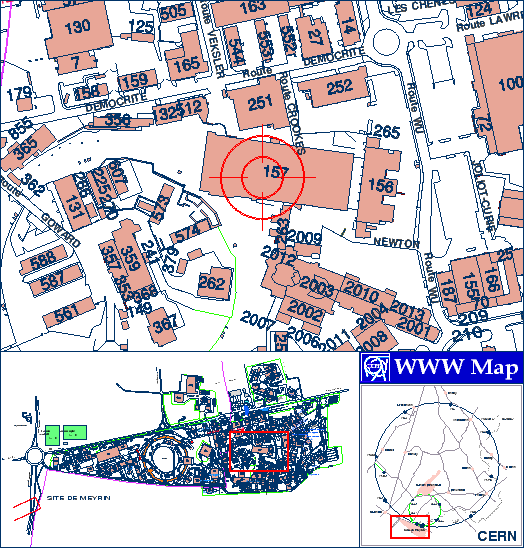
\includegraphics[width=0.6\textwidth]{./images/meyrin_map_157}
	\caption{A map of the CERN Meyrin site showing the location of building 157, where the IRRAD and CHARM facility are located (\url{http://building.web.cern.ch/building/})}
	\label{fig:meyrin_map}
\end{figure}

\begin{figure}[!ht]
	\centering
	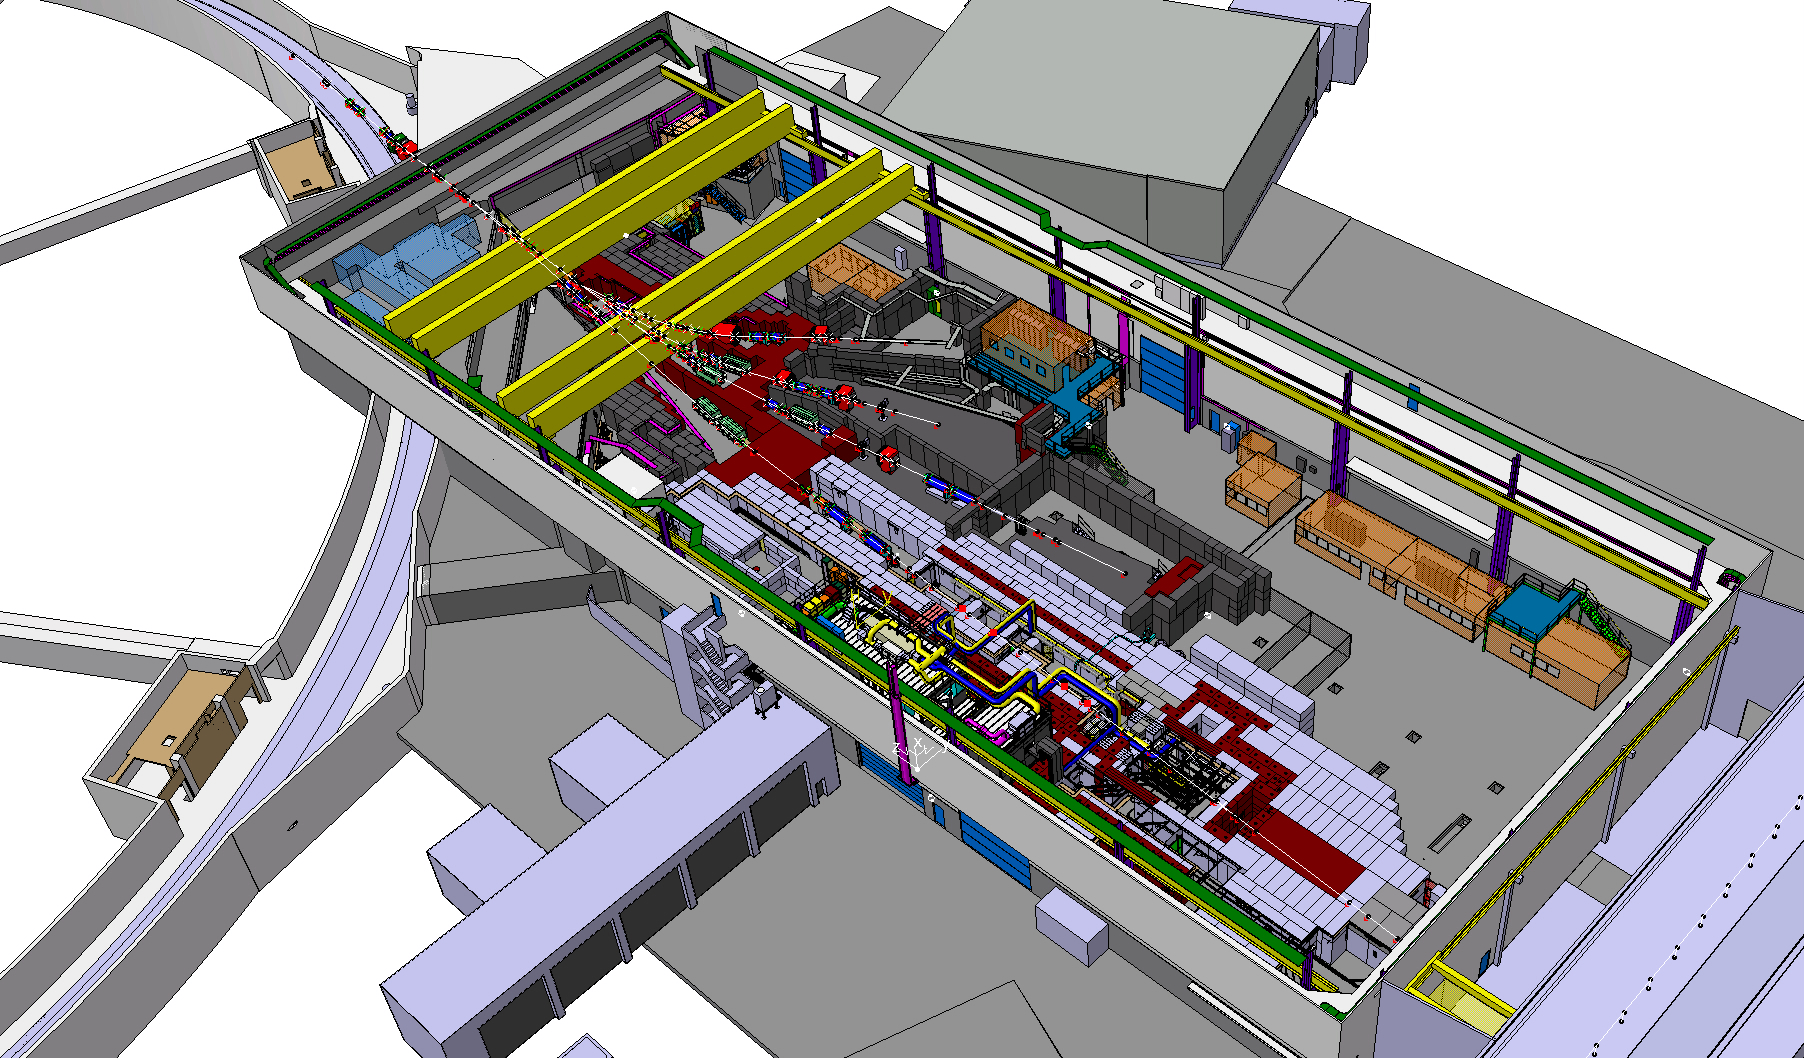
\includegraphics[width=0.9\textwidth]{./images/EastArea-Vue3D-1}
	\caption{A screen-shot from the 3D drawing of the PS East Area Hall. The IRRAD and CHARM facility are located in the southern part of the hall (bottom-right of the image).}
	\label{fig:eastarea_hall_3d}
\end{figure}
%\documentclass[main.tex]{subfiles}
%\begin{document}

\section{Facility Description}

The CHARM facility consists of a main test area (also referred to as target area), 2 control rooms and a buffer-area for storage \footnote{A more detailed description of the facility can be found in the safety file \cite{charm_safety_file}.}. A layout drawing of the T8 beam-line and surrounding areas is shown in figure \ref{fig:irrads_layout}, and a photo of the test area is shown in \ref{fig:test_area_photo}. The main (larger) control room is dedicated to monitoring the facility and has space for users to make dry-runs of their test set-up, whereas the technical-locale is where the control and monitoring equipment for the users is installed during their tests. A separate platform outside the control room is available for testing large devices (full sized racks and large equipment) which connects directly with the control room for dry-testing. All the connections and cabling (including length) within the control match exactly those used between the test area and technical-locale, as to keep the dry-run set-up configuration exactly the same as with the real tests.  \\

To perform a test, the users device is installed on a rack and moved to the test positions using an automated conveyor system (AVT). The test positions are shown in figure \ref{fig:fluka_test_positions}.  The cabling for the test device is placed into a 'cable-order-chain' attached to a rail system and is moved in to place together with the conveyor. Figure \ref{fig:cable_chain} shows how the cables are arranged. Inside the test area there is a patch-panel with an array of different connections for the user to connect their equipment. These connections lead directly to a patch-panel inside the technical locale. A list of available cables and connectors can be found on the CHARM website: \url{http://charm.web.cern.ch/CHARM/Cables.php} \\

During operation the beam is directed on one of three targets; copper, aluminium and 'aluminium with holes'. By choosing different targets, the intensity of the radiation field can be varied, with the copper target generally giving the highest dose and particle fluences, and the 'aluminmium with holes' target giving the least dose compared to the other targets. For in beam measurements it is possible to run without target, so one can test in a 24 GeV proton field. \\

There are four layers of shielding installed in the middle of the area which can be moved in and out of place to tailor the radiation field. The outer two layers of 20cm thick concrete surround two layers of 20cm thick iron in a 'sandwich' arrangement. The 'concrete-iron-iron-concrete' layout is referred to as 'CIIC' for the facility configuration, where partial shielding and running without any shielding at referred to as 'CIOO' (concrete-iron-open-open) and 'OOOO' (all four open). \\

Within the test area there are a number of different positions one can place test equipment in CHARM, which can either be directly in the proton beam, behind shielding or at various angles and distances from the target. These are either at the designated test positions or at the Montrac positions. By varying the target, shielding and position of the test device, a large number of radiation fields can be achieved. These are described in detail in chapter 3. \\

\begin{figure}[ht!]
	\centering
	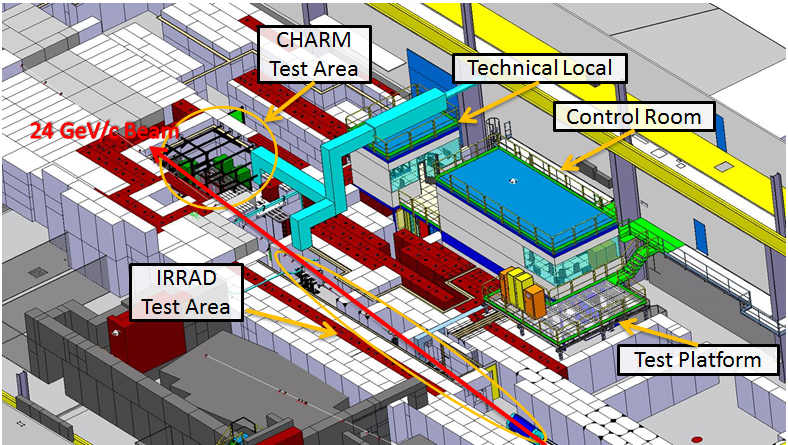
\includegraphics[width=0.8\textwidth]{./images/charm_overall_ann}
	\caption{A screen-shot from the 3D Catia drawing of the IRRAD and CHARM facility, showing the different areas.}
	\label{fig:irrads_layout}
\end{figure}

\begin{figure}[!ht]
	\centering
	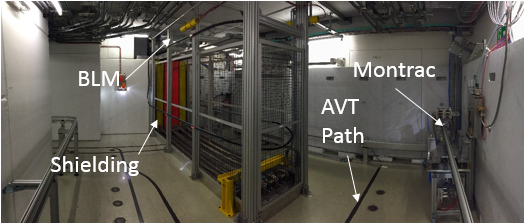
\includegraphics[width=\textwidth]{./images/test_area_photo_ann}
	\caption{A photo of the test area. The moveable shielding is in the centre of the photo, with the target behind.}
	\label{fig:test_area_photo}
\end{figure}

\begin{figure}[ht!]
	\centering
	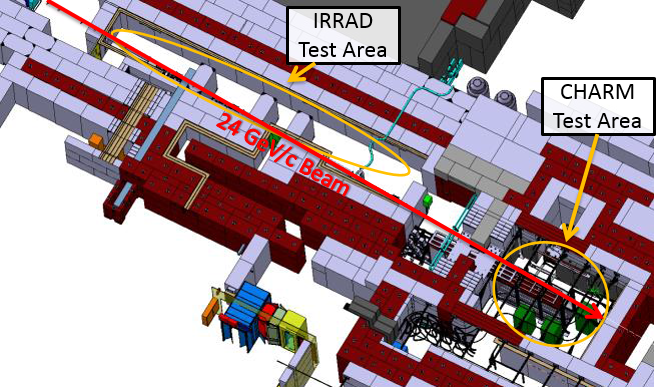
\includegraphics[width=0.8\textwidth]{./images/irrad2}
	\caption{A screen-shot of the 3D Catia drawings for the T8 beam-line on the East Area hall showing the position of the IRRAD and CHARM facilities along the T8 beam-line.}
	\label{fig:t8_screenshot}
\end{figure}

\begin{figure}[!ht]
	\centering
	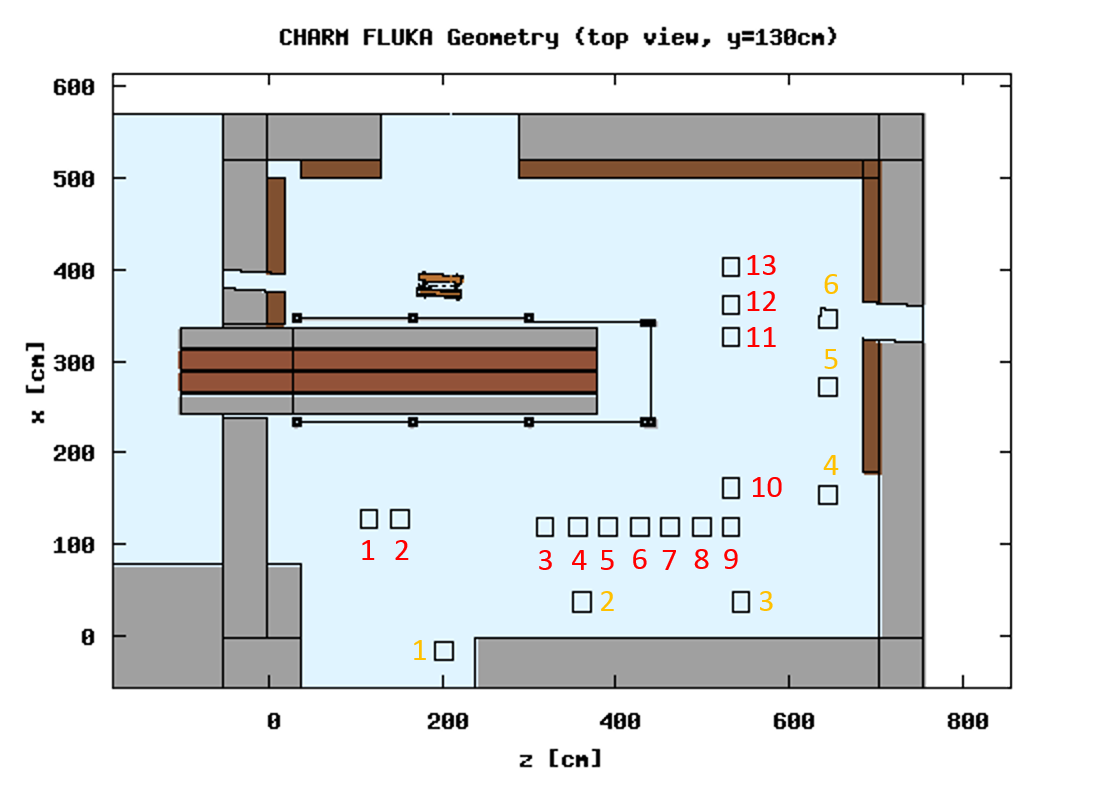
\includegraphics[width=0.8\textwidth]{./images/test_pos_new_ann}
	\caption{A screen-shot showing the test positions in the FLUKA geometry, cut at beam-height. The rack positions are numbered in red, and the Montrac test positions are numbered in yellow.}
	\label{fig:fluka_test_positions}
\end{figure}

\clearpage
\subsection{Facility Configuration}

There are a number of possible ways to change the radiation field within the test area depending on the requirements of the users and the desired test environment. Below is a list of the options.

\begin{description}
\item[Targets] \hfill \\
There are 3 targets for use in the test area; copper, aluminium and aluminium with holes. The first 2 are solid metal, however the third is made from machined disks of aluminium with cuts made through the centre, reducing the effective density along with middle by a factor 2, leading to less beam interaction. These are referred to as 'cp', 'al' and 'alh' respectively.

\item[Shielding] \hfill \\
Between the test positions and target inside the test area, there are 4 movable shielding plates, made of either concrete ('C') or iron ('I'). The configuration of the shielding is referred to in the calculations as the order starting closest to the target and going further away. An example is 'CIIC', which means all shielding is in place, alternatively there are 'CIOO' which means half shielding, and 'OOOO' which means no shielding being used. 

\item[Test Positions] \hfill \\
%to do! update with 13 new positions
These are the 'rack' test positions, for which a conveyor system will be used to move the racks filled with the test electronics. There are a total of 13 possible rack positions, which will be referred to as 'r1' to 'r13'. These are in the mixed-field. The positions shown in figure \ref{fig:fluka_test_positions} and the coordinates relative to the FLUKA geometry are described in the appendix in table \ref{tab:test_positions}.

\item[Beam Conditions] \hfill \\
The beam extracted from the PS can be altered in a number of ways to suit the needs of the users. Firstly considering the effective beam intensity reaching the facility, the spill size and frequency can be altered. This can be varied from around 1E11 up to 5E11 per spill with up to 6 spills per super-cycle, giving around a factor 30 range in intensity for the users. More details on the beam conditions are given in the following section. \\
\end{description}

\noindent In addition to the above, there are other special test positions available: \\

\begin{description}
\item[Montrac Positions] \hfill \\
% to do! 
These are positions along the Montrac rail system where the shuttle can stop and one can leave the equipment to be irradiated. There are fewer positions that the usual test locations, but adds additional positions for smaller equipment that can be run in parallel with the large racks. A photo of the Montrac test location is shown in figure \ref{fig:montrac_testbox}.

\item[In-beam Position] \hfill \\
In addition to the Montrac positions, it is possible to stop the shuttle directly in beam and leave equipment for testing.
\end{description}

\begin{figure}
\centering
\begin{subfigure}{.5\textwidth}
  \centering
  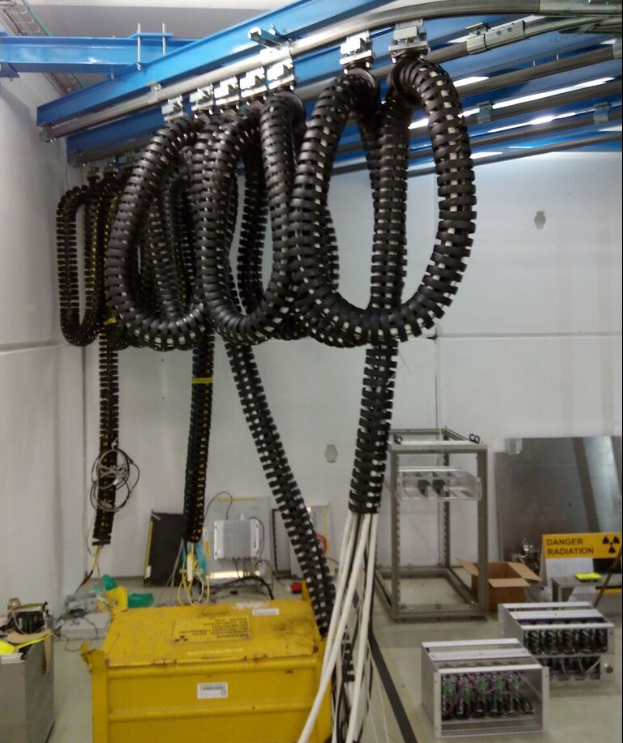
\includegraphics[width=.9\linewidth]{./images/cable_chain_storage}
  \caption{}
  \label{fig:cable_chain1}
\end{subfigure}%
\begin{subfigure}{.5\textwidth}
  \centering
  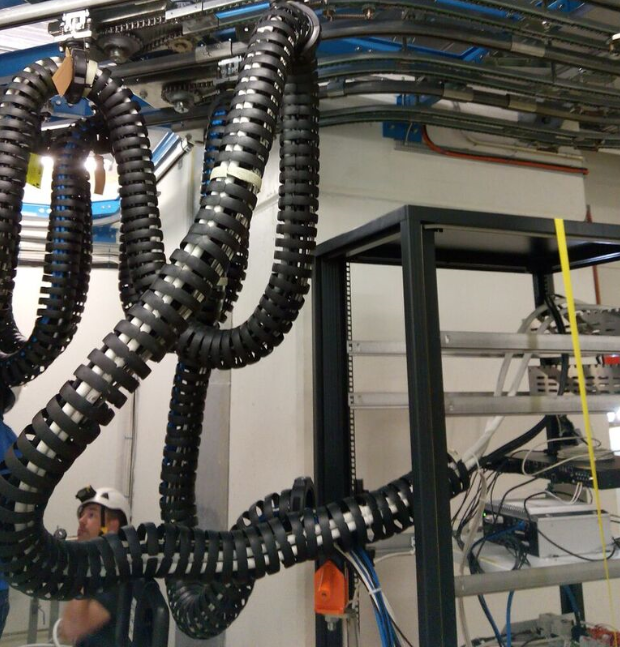
\includegraphics[width=.9\linewidth]{./images/cable_chain_to_rack}
  \caption{}
  \label{fig:cable_chain2}
\end{subfigure}
\caption{A photo of the cable-order-chain used to keep all the user cables together, and runs on a rail system making it easy to manipulate a potentially heavy mass of cables. Photo (a) shows the cable within the storage area, and photo (b) shows a test rack being connected to the cables.}
\label{fig:cable_chain}
\end{figure}

\begin{figure}[!ht]
	\centering
	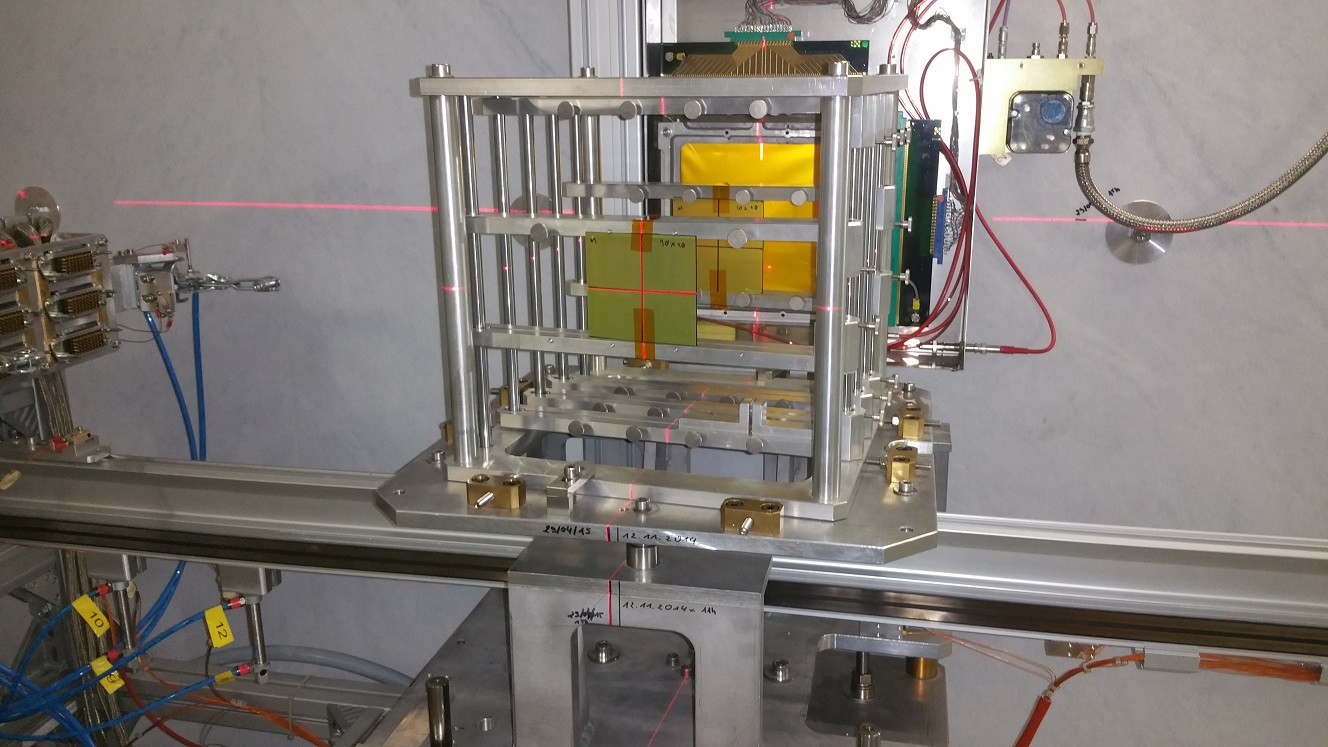
\includegraphics[width=0.8\textwidth]{./images/montrac_testbox2}
	\caption{A photo of the Montrac test location with the test rack in place, ready for in-beam tests.}
	\label{fig:montrac_testbox}
\end{figure}


% beatch file in appendix

\clearpage
\subsection{Beam Instrumentation}
For monitoring the beam reaching the IRRAD and CHARM test facilities, there are a number of instruments that can be used to measure the beam intensity, position and size. All the available monitors are shown in figure \ref{fig:t8_instrumets}. The instrumentation falls into 2 categories; \textbf{intensity monitoring}, and \textbf{position and beam size monitoring}. \\

\subsubsection{Beam Intensity Monitoring}

The beam intensity can be measured using either of the secondary emission counters (SEC1 and SEC2) or the ionisation chamber (IC). \textbf{To determine the number of protons reaching the target (POT) at CHARM, the SEC1 detector is to be used as the reference.} This detector is calibrated using the 'fast beam current transformer' (BCT) placed up-stream, just after the point of extraction from the PS. A cross-check is also made using activation foils. \\

During the SEC1 calibration tests \cite{pozzi2015} a calibration factor of 1.84E7 protons per SEC1 count was found using an activation foil method. This is the value that will be used to normalise experimental results to compare with the FLUKA calculations. \\

The SEC2 can also be used to measure the POT, however as this detector is positioned after the IRRAD facility, the signal can be influenced by sampled placed in beam at IRRAD. This has been observed during operation and can give misleading beam intensity measurements (reference), therefore it is recommended to use the SEC1 for POT calculations. The data from the SEC1, SEC2 and IC are all continuously logged in TIMBER. The variable names are listed in table \ref{tab:beam_instruments}. \\

\subsubsection{Beam Position and Size Monitoring}

The position of the beam can be measured as it passes through IRRAD using the 'beam position monitors' (BPM) (\url{https://ps-irrad.web.cern.ch/irrad/bpm.php}) and with the 'beam TV' (BTV) or 'multi-wire proportional chamber' (MWPC) as it passes CHARM. The BTV is only used to verify the beam position is correct after changes on the T8 beam-line. During operation the MWPC is used to monitor the beam shape and position. The detector is placed at the back of CHARM, just behind the Montrac test position. The data is logged in TIMBER under the variable names described in table \ref{tab:beam_instruments}. \\


\begin{table}[h!]
	\begin{center}
	\begin{tabular}{l|l}
	Detector & TIMBER Variable Name \\ 
	\hline 
	\hline
	SEC1 &  MSC01.ZT8.107:COUNTS \\ 
	SEC2 & MSC02.ZT8.125:COUNTS  \\ 
	IC & ION01.ZT8.124:COUNTS \\ 
	MWPC (x) & MWPC.ZT8.135:PROFILE\_H \\ 
	MWPC (y) & MWPC.ZT8.135:PROFILE\_V \\ 
	\end{tabular}
	\end{center}
	\caption{A table of the variable names as used in the logging database for the various beam instruments. The 'ZT8' refers to the T8 beam-line, and the number proceeding it refers to the distance of the detector to the beam extraction from the PS.}
	\label{tab:beam_instruments}
\end{table}

\begin{figure}[!ht]
	\centering
	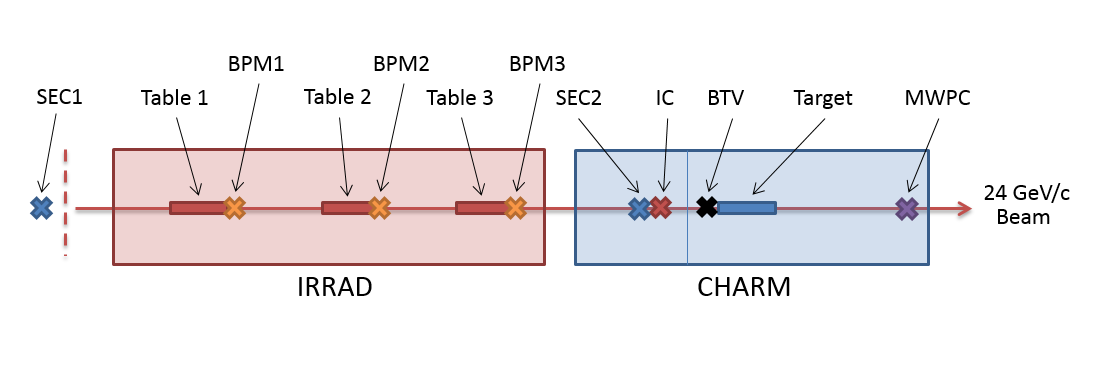
\includegraphics[width=\textwidth]{./images/beam_layout}
	\caption{A diagram of the beam instrumentation for the T8 beam-line.}
	\label{fig:t8_instrumets}
\end{figure}

\subsection{Beam Specification}

The CHARM facility receives a 24 GeV/c proton beam extracted from the CERN proton-synchrotron (PS), which is directed along the T8 beam-line in the PS East-Area Hall towards CHARM. The beam structure is in 'spills' (or bunches) of length 350ms, separated by 1.2 seconds and ordered in a 'super-cycle' usually of around 30 spills. This gives the beam a 'burst' like nature, as opposed to a constant beam without interruption. Each user of the beam is allocated a specific spill (or several spills) and these are extracted individually to the respective beam-lines. An example of how the spills are typically arranged can be seen in figure \ref{fig:ps_vista}. \\  

The beam conditions for the T8 beam-line can vary based on the different parameters used from extraction down to the magnets preceding the IRRAD facility. For the cases when the target is being used, the beam will be focused on the target, with a FWHM of around 3cm. For direct irradiation in the beam, it is possible to enlarge the beam up to a FWHM of 10cm. More information about the  beam parameters and conditions can be found in the T8 beam specification document \cite{Gatignon2013}. A summary of the usual beam conditions is shown in the next section. A detailed report on the beam characteristics during the enlarged beam size has been made available on EDMS \cite{charmblown}.\\

\begin{figure}[!ht]
	\centering
	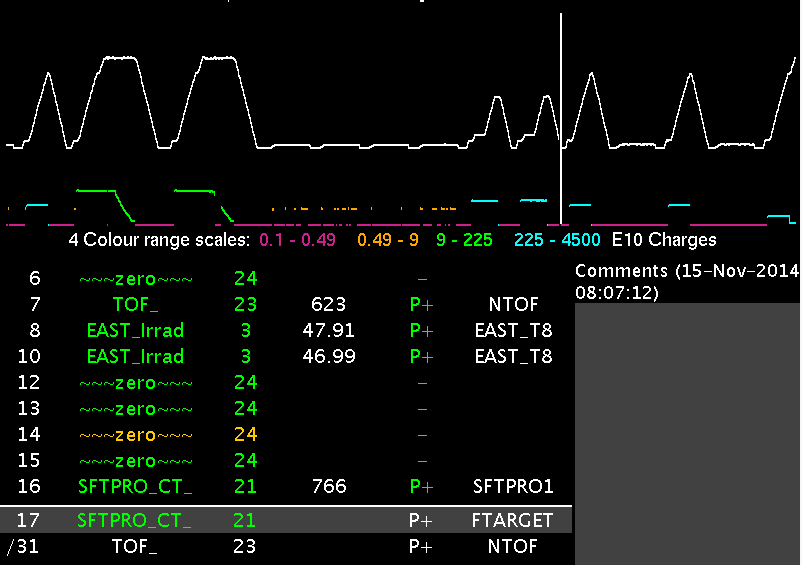
\includegraphics[width=0.6\textwidth]{./images/vistar_example}
	\caption{A screen-shot of the PS VISTAR page, giving live information about the beam extracted from the CERN PS. In this example, CHARM is receiving 2 spills (numbers 8 and 10) from a super-cycle of length 31 spills. The intensity measured at extraction in this case is around 4.7E11 protons per spill.}
	\label{fig:ps_vista}
\end{figure}

\subsection{Operating Conditions}

During the initial test period in October 2014, an analysis was made of the average beam intensity. It was possible to determine the average spill size and frequency, which can be used to make an estimate for the number of POT impinging the target over a set period. It was found that the average intensity seen on the SEC1 was 3.1E11 protons per spill. It was also noted that there was typically 3 spills per minute, which gives an average of around 1.8E10 protons per second, or 1.5E15 protons per day of running. This assumes no break in operation and no changes in the beam conditions. Therefore, to use a reasonable scaling value for the remaining document, \textbf{1.5E15 protons per day} will be assumed when normalising datasets, and will be referred to hereafter as the nominal operation conditions. \\

During the same period it was noted that the spill frequency can be varied from 1 to 6 spills per minute, and the spill intensity can vary from 1.5E11 to around a maximum of 4.0E11 protons per spill. This gives the lower and upper running limits of around 2.1E14 to 2.3E15 protons per day respectively. \\

The beam size for irradiation with the target uses the normal beam conditions from the PS, which gives a beam-size of around 1 to 2cm FWHM at the target. For in beam tests, it is possible to request the 'blown-up' beam setting from the PS operators. The reference for this was set during tests on 01/06/2015, and a beam of 8cm FWHM in the horizontal plane, and 12cm FWHM in the vertical was achieved. A plot of this on the MWPC is shown in figure \ref{fig:beam_reference2}. The values for the beam reference can be found in table \ref{tab:mwpc_reference_values}. \\

The beam profile on the BPM1 was analysed for the test periods over November and December 2014 and an average made over all channels in the x and y planes. It was seen to have a Gaussian distribution, with a FWHM of 14.6mm and 10.7mm in x and y respectively. The profile differed slightly for BPM2 where the beam was larger in the y plane, with a FWHM of 11.5mm and 14.1mm in x and y respectively. \\

%to do! update with the reference conditions (see e-mails)
\begin{table}[!ht]
\begin{center}
	\begin{tabular}{c|c|c|c|c}
	\textbf{Beam Setting} & \textbf{Units} & \textbf{x Plane} & \textbf{y Plane} & \textbf{Tolerance} \\ 
	\hline 
	\hline 
	With target			& mm	& 22	& 22	& $\pm$3 \\ 
	Without target		& mm	& 80	& 120	& $\pm$10 \\ 
	\end{tabular}
\caption{Table of the reference beam settings for CHARM, as measured with the MWPC, for use with and without target (blown-up beam).}
\label{tab:mwpc_reference_values}%
\end{center}
\end{table}

\begin{table}[!ht]
\begin{center}
	\begin{tabular}{l|c|c|c}
	\textbf{Data} & \textbf{Units} & \textbf{Value} & \textbf{Tolerance}\\ 
	\hline 
	\hline 
	PS Vista spills & spills/SC & 3			& $\pm$2 \\
	SEC1 			& p/spill	& 3.60E+11 	& $\pm$5E10 \\
	BPM1 (centre) 	& mm		& 0			& $\pm$5 \\
	BPM1 (sigma)	& mm		& 8			& $\pm$5 \\
	MWPC (centre)	& mm		& 0			& $\pm$5 \\
	MWPC (FWHM)		& mm		& 22*		& $\pm$20 \\
	\end{tabular}
\caption{A table of the typical parameters for the various monitors and detectors used at CHARM. These are for when the target is not in use. Details on the blown-up can be found in a dedicated report \cite{charmblown} \\ * note this will increase to around 80mm when the target is in place.}
\label{tab:monitor_reference_values}%
\end{center}
\end{table}

\begin{figure}[!ht]
	\centering
	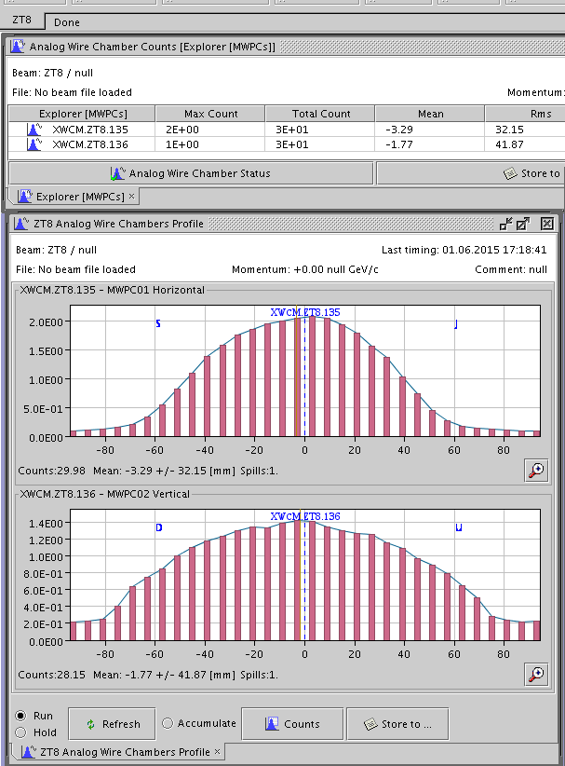
\includegraphics[width=0.6\textwidth]{./images/blown_up_beam}
	\caption{A screen-shot of the CESAR tool, showing the MWPC profile during the 'blown-up' beam reference conditions.}
	\label{fig:beam_reference2}
\end{figure}

\begin{figure}[!ht]
	\centering
	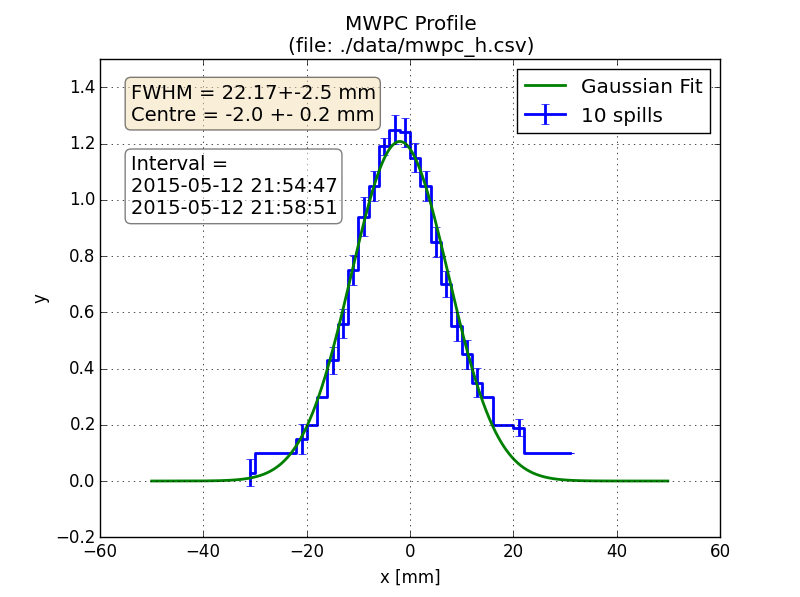
\includegraphics[width=0.6\textwidth]{./images/mwpc_com_10spills}
	\caption{A plot of the horizontal beam profile captured with the MWPC during the commissioning period. This is the typical beam used with the target.}
	\label{fig:mwpc_profile}
\end{figure}

\begin{figure}[!ht]
	\centering
	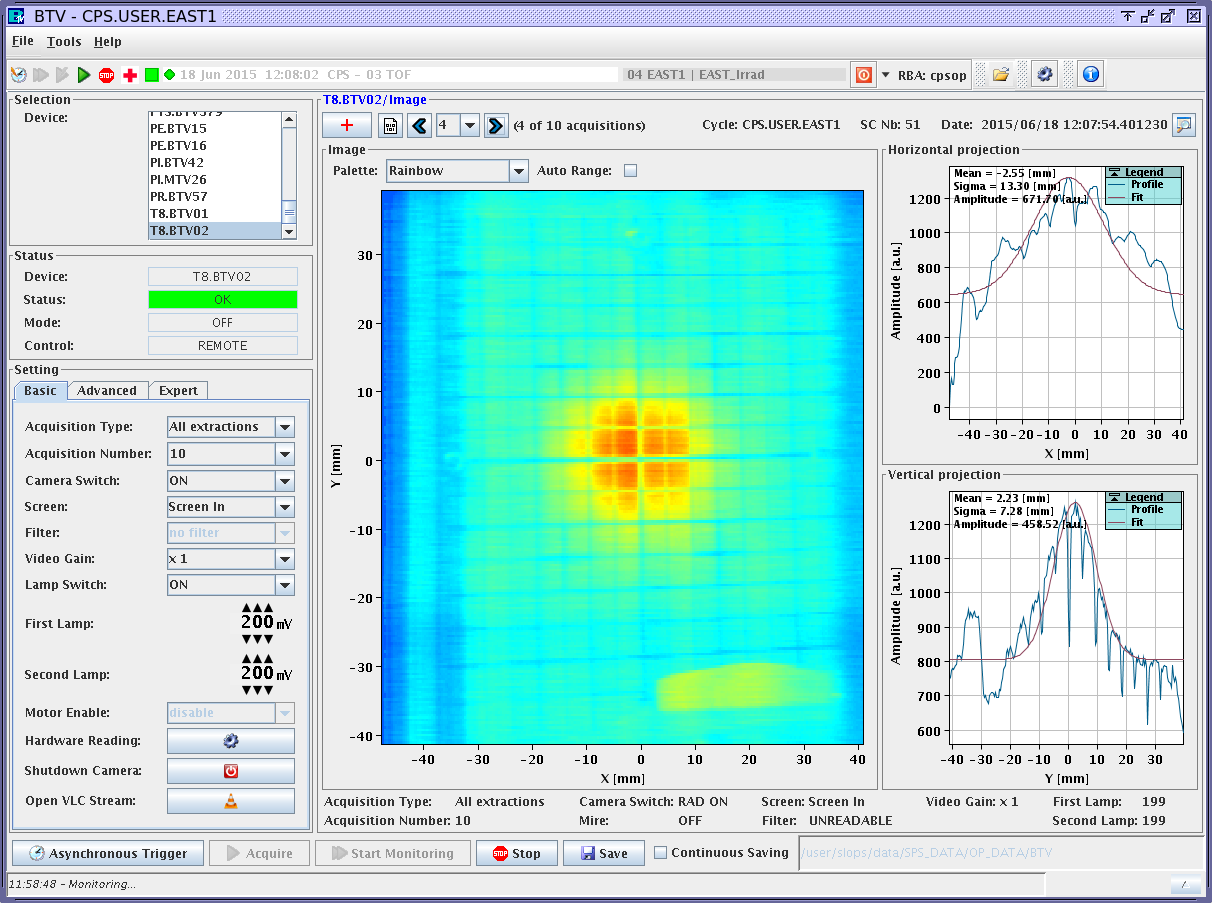
\includegraphics[width=0.5\textwidth]{./images/btv_example}
	\caption{An example of the BTV acquisition from the PS operators showing the spill alignment. In this case, the beam was aligned perfectly.}
	\label{fig:btv_example}
\end{figure}

\begin{figure}[!ht]
	\centering
	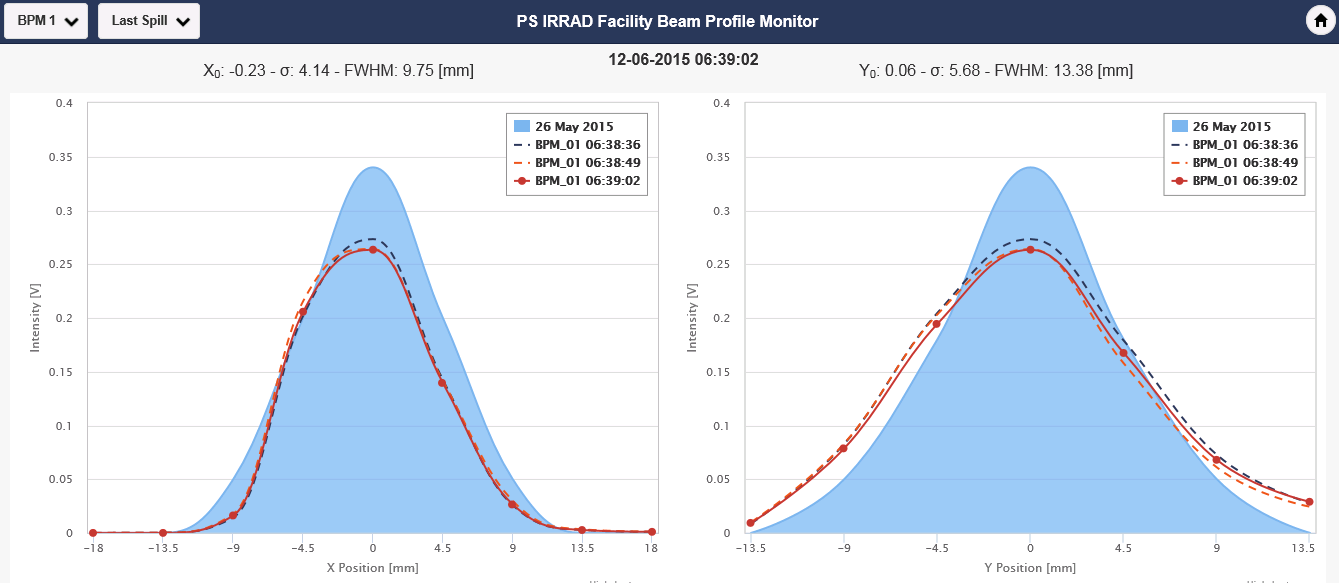
\includegraphics[width=0.8\textwidth]{./images/bpm_example}
	\caption{Example plots of the BPM1 from a typical testing period. The BPM1 is the reference when aligning the beam before using the target.}
	\label{fig:bpm_example}
\end{figure}

\begin{figure}[!ht]
	\centering
	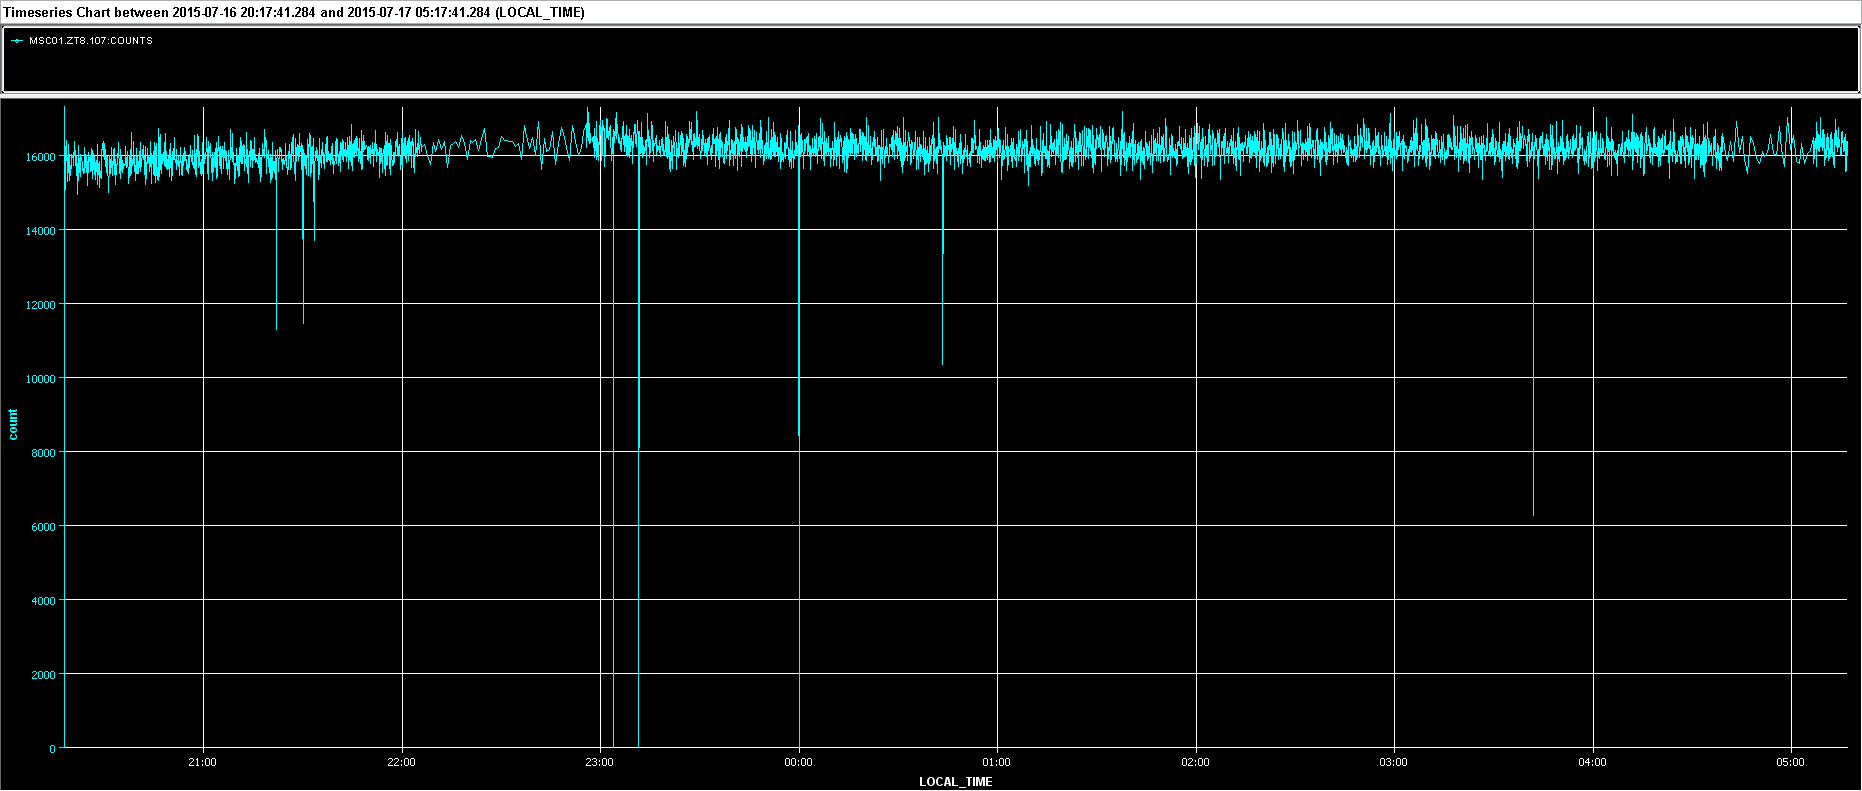
\includegraphics[width=0.8\textwidth]{./images/sec1_example}
	\caption{An example of the SEC1 signal acquired from TIMBER showing the beam intensity over a certain period.}
	\label{fig:sec_example}
\end{figure}
%\documentclass[main.tex]{subfiles}
%\begin{document}

\section{Radiation Field}

This chapter describes the radiation field inside the CHARM test area. With the many different facility configurations, there is a large variation in the particle and energies seen in the spectra at the various test locations. In order to understand what the field is like in the different test positions, the FLUKA Monte Carlo code has been used to simulate the radiation field. This starts with making an accurate model of the inside of the test area, correctly describing the beam and making reasonable assumptions about the running of the facility. \\

In order to make a thorough and complete analysis of the radiation field, it is important to decide what information is needed, and how it can be compared with real-life mixed radiation fields such as space or accelerator facilities. This step requires the formation of metrics and standards, in order to make accurate comparisons and consider the strength of the match. From there, tables of data can be produced for each position and each configuration, stating the matches for various comparisons. \\

A list of useful units is included in the appendix, table \ref{tab:useful_quantities}. \\

\subsection{Quantifying the Radiation Field}

There are many quantities which are useful to know during radiation tests, and these vary depending on the kind of test a user would like to make. It ranges from the simplest total ionising dose (TID) tests, where only the dose at the location as a function of time is needed, to very specific quantities such as 1MeV equivalent neutron fluence which is useful in studies of displacement damage in electronics. \\

The radiation environment inside the CHARM area is described as a 'mixed' field. This means that the radiation within the test area comes in many types, such as protons, neutrons, pions, etc, and of a wide range of energies. These originate from the beam interacting with the target. This is contrary to a gamma facility for example, where the field is only 1 type of radiation. In fact many radiation environments can be described as a mixed-field, such as in the upper atmosphere where one finds not only protons but also neutrons and muons, thus the types of radiation are 'mixed'. \\

At CHARM one can find an entire range of particles from the beam interaction with the target. At the test location one typically sees a number of hadrons (including protons, neutrons, pions and kaons), leptons (electrons, positions and muons) and photons (x-ray and gamma). These range in energy from near primary beam protons and neutrons at 24 GeV, to thermal neutrons from the test area wall scattering at \textless 1 eV. \\

\subsection{Metrics}

In order to compare the mixed-radiation field at CHARM with other fields, a metric needs to be defined in order to be able to describe and then compare radiation fields. This should give a clear and simple way to cross-compare, and should also show the strength of the fit. This could be either a single value, or a number of different tests that overall show the quality of the fit for that environment. \\

There are potentially many ways to compare different mixed radiation fields. There are fluences of various different particles of which have a variety of types and energies, all which have varying impacts on the operation of electronics and systems containing electronic components. To narrow the search down, one key factor that is important for SEEs is particle energy, and how it transfers the energy to sensitive part of the device. A measure of this is the 'linear energy transfer' (LET), and usually there is a minimum LET required to induce SEEs (depending on the specific device or system). To further narrow the search, typically the only kind of particles that can cause reactions which produce particles with LETs large enough to cause SEEs are hadrons. Therefore the area of interest for SEEs in electronics is usually hadrons with a high enough energy (LET) to cause the problems we are trying to avoid \cite{rad_effects_handbook}. \\

% Explain HEH, HEHeq, r, n_thrm

Before introducing the metrics describing the radiation field, it is important to define some quantities used in the metrics. The first is called the 'high-energy' hadrons (HEH), which corresponds to all hadrons above an energy of 20 MeV. This particular energy is chosen since this energy corresponds to a rough minimum required to cause SEEs. There is a second similar value called the high-energy hadron equivalent (HEHeq). The difference lays in the way the fluence of hadrons below 20 MeV is calculated. In this case, instead of a minimum threshold, a Weibull function is used to model the response of a typical SRAM used for SEU detection (in the Radmon system for example). This response is then assumed to be more accurate than the former method for defining the HEH fluence. \\ 

Two further values of interest that can be helpful when defining the metrics are the 'r factor' and the thermal neutron equivalent fluence. The r factor (or risk factor) is the ratio between the fluence of thermal neutrons to HEH. Since thermal neutrons can cause problems due to the ionisation of products of nuclear capture reactions within the electronics, it is important to define their contribution from the overall hadron fluence \cite{Baumann2001211}. The sensitivity of electronics to thermal neutrons is not always well tested for, and thus the risk of placing electronics in a field that contains thermal neutrons is very useful to know. The r factor can be calculated using the Radmon system by making multiple measurements at a specific location with different detector biases \cite{Kramer:1399765}. \\

The thermal equivalent fluence is calculated by taking the thermal neutron fluence and folding with a 1/v weighting to replicate the capture cross-section of neutrons in boron 10. This is relevant to studies of SEEs in electronics since boron 10 was previously found in a number of electronic components due to certain manufacturing processes and the products from the nuclear reactions have a high enough LET to induce SEEs \cite{Baumann2001211}.\\

The first metric that could be used are the 'hardness factors', which quantify range of energies of high energy hadrons in a radiation environment. To calculate these factors, one takes the simulated high energy hadron spectrum and makes a reverse integral, normalised to 1 at 20MeV. From this, the values at 50\% and 10\% (H50 and H10) are taken, which correspond to the proportion of the HEH fluence above this energy. \\

A second way to make a comparison between data-sets and real measurements could be to use the fission cross-section in Tungsten for devices where the material is used. The importance of Tungsten is from the fragments caused during fission reactions. These fragments have a large LET and thus deposit large amounts of charge, which maybe be close to the active volume of the electronics \cite{1589248}. \\

The method involves taking the simulated proton-induced Tungsten fission cross-section and folding this with the simulated normalised HEH fluence. The integral of the folded spectrum will give the probability of a fission event in Tungsten for this HEH spectrum. For a comparison with a real value, one can divide this by the 230 MeV proton induced fission cross-section in Tungsten. Then, if one tests a device in a 230 MeV proton beam, the ratio will give an indication of how the number of events could scale in the simulated HEH spectrum. An example of this method is shown in figure \ref{fig:w_factor_example}, which gives a ratio of 1.322 between the expected cross-section in the mixed-field at this location and configuration and the cross-section at 230 MeV. \\

\begin{figure}[!ht]
	\centering
	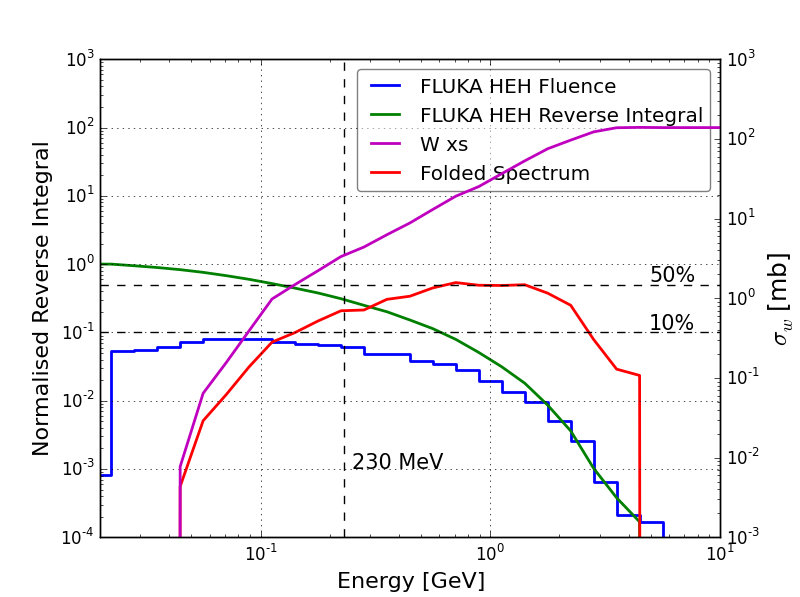
\includegraphics[width=0.7\textwidth]{./images/w_folded_spectrum3}
	\caption{A plot of the HEH fluence for a specific test position, folded with the Tungsten fission-fragment cross-section, giving a 'response' for a detector in which the SEU sensitivity is dominated by the Tungsten inside the device. A reference of 230 MeV is used to compare with results with those obtained during tests at PSI in Switzerland. Also plotted is the HEH reverse integral spectra, with the corresponding H10 and H50 factors.}
	\label{fig:w_factor_example}
\end{figure}

\clearpage
\subsection{Standards and Environments}

There are a number of different environments (natural or otherwise) which have been studied to calculate the radiation field. The different radiation types, energies and fluences are calculated  for each environment and tabulated, but to be able to compare them, some standards have to be created. As shown in the previous section, one way to compare different mixed-field radiation environments is to use the 'hardness-factor' which is related to the fluence of high-energy hadrons, and gives information about the energy and flux of hadrons. A collection of these values, including spectral information is shown in table \ref{tab:hardness_energies}. The data for the various LHC areas is given for nominal conditions (50fb$^{-1}$). \\

%For TID testing, there are a range or standard dose rates... (need table) ELDR..\\

%Description and reference to some different environments (spectra plots?) \\

\begin{table}[htbp]
\small
  \centering
    \begin{tabular}{l|p{1.8cm}|r|r|r|r|r|r|r|r}
    \textbf{Environment} & \textbf{HEH /cm$^{2}$/ y} & \multicolumn{4}{c|}{\textbf{Composition (\%)}} & \textbf{R} & 				\multicolumn{3}{c}{\textbf{Hardness Energy}} \\ \cline{3-6} \cline{8-10}  
    & & n & p & pi$^{+-}$ & n$_{int}$ & & H50 & H10 & H1 \\
    \hline
    \hline
    CERN - LHC UJ 				& 2.5E+09 & 99    & 1     & 0     & 32    & 2     & 0.08  & 0.18  & 0.36 \\
    CERN - LHC RR 				& 1.0E+09 & 71    & 13    & 16    & 25    & 10    & 0.18  & 0.69  & 2.8 \\
    CERN - LHC Tunnel 			& 6.0E+11 & 45    & 18    & 37    & 19    & 2.8   & 0.37  & 1.8   & 5.7 \\
    CERN - ATLAS Outer Tracker 	& 3.5E+09 & 67    & 5     & 28    & 25    & 1.1   & ?     & 0.46  & 0.71 \\
    CERN - ATLAS Inner Tracker 	& 1.0E+12 & 4     & 7     & 89    & 1     & 2     & 1.5   & 3.8   & 12 \\
    CERN - LINAC 4 				& 1.0E+10 & 99    & 1     & 0     & 86    & 1.5   & ?     & 0.07  & 0.1 \\
    CERN - PS 					& 1.0E+11 & 61    & 17    & 22    & 19    & 4.9   & ?     & 0.9   & 2.4 \\
    CERN - SPS 					& 1.0E+12 & 70    & 12    & 18    & 29    & 48.9  & ?     & 0.94  & 5.1 \\
    QARM - 350m (Geneva, CH) 	& 1.6E+05 & 93    & 7     & 0     & 21    & 0.12  & 0.08  & 0.34  & 1.3 \\
    QARM - 10km (Geneva, CH) 	& 1.7E+07 & 82    & 18    & 0     & 18    & 0.08  & ?     & 0.92  & 5 \\
    QARM - 20km (Geneva, CH) 	& 3.8E+07 & 68    & 32    & 0     & 14    & 0.06  & 0.5   & 2.9   & 13 \\
    CREME 96 - ISS (450km) 		& 7.3E+08 & -     & -     & -     & -     & -     & ?     & 0.25  & 0.53 \\
    CREME 96 - Proba II (800km) & 2.7E+09 & -     & -     & -     & -     & -     & 0.1   & 0.28  & 1.5 \\
    \end{tabular}%
  \caption{Table of hardness energies for various radiation environments \cite{radecs2014shortcourse}. The hardness factors for the spectra calculated with CREME96 used protons only. The 'n$_{int}$' component stands for the intermediate neutrons, which are those with an energy between 0.2 MeV and 20 MeV. The hardness energies are given in GeV.}
  \label{tab:hardness_energies}%
\end{table}%

% 1E9 HEH = approx 1 Gy. These are from the nominal conditions. Hi-Lumi factor 10? Starting 2024 (after LS3) \\

%Add a column of dose rates per year to compare \\

%Add the references to the LHC areas (for example, which UJ does this refer to?) \\





\newpage
\subsection{FLUKA Calculations}

The FLUKA Monte Carlo code \cite{FLUKA1} \cite{FLUKA2} was used to perform the radiation field calculations for the CHARM test area. For this, a geometry was built specifically for CHARM test area. This geometry includes all the main features of the test area; i.e. the target table with the 3 different targets, the movable shielding, the different materials in the surrounding shielding walls, the exact test positions etc. An effort was made to make the geometry as accurate as possible with respect to the technical drawings and double-checked with measurements made in the facility, in order to reduce the errors with respect to positioning. Care needed to be taken as the variations in the radiation field with respect to position (gradients) can be high for areas close to the beam and down-stream of the target. \\

\subsubsection{FLUKA Geometry}

An accurate model was made specifically using FLUKA for the CHARM area. Details and dimensions were taken from a combination of CATIA 3D drawings, and then finally measurements once the facility had been constructed. It was decided to focus on the details around the test area, therefore the geometry as seen in FLUKA includes only the first layer of shielding. This will optimise the time used during the calculations by not tracking the particles in area that are not of interest. \\

The co-ordinate system for the FLUKA geometry was defined with the z axis parallel with the beam, y axis for the height, and the x axis adjacent to the beam. This will then be used in the rest of the document when describing the radiation field. These along with the test positions can be seen in figure \ref{fig:fluka_test_positions}.\\


\begin{figure}[!ht]
	\centering
	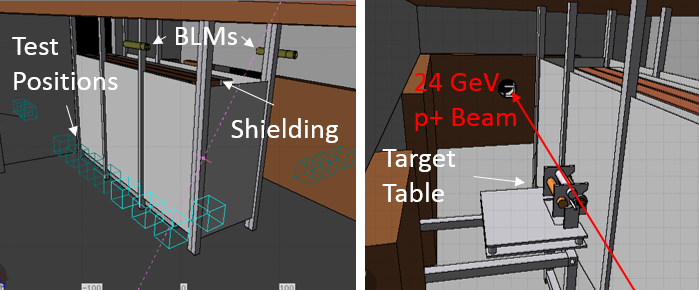
\includegraphics[width=0.9\textwidth]{./images/fluka_charm_shielding_ann2}
	\caption{A screen-shot of a cut of the FLUKA geometry, showing the shielding and test position scorings (in blue). The BLMs are also visible at the top of the shielding.}
	\label{fig:fluka_screenshot}
\end{figure}

\begin{figure}[!ht]
\centering
\begin{subfigure}{.5\textwidth}
  \centering
  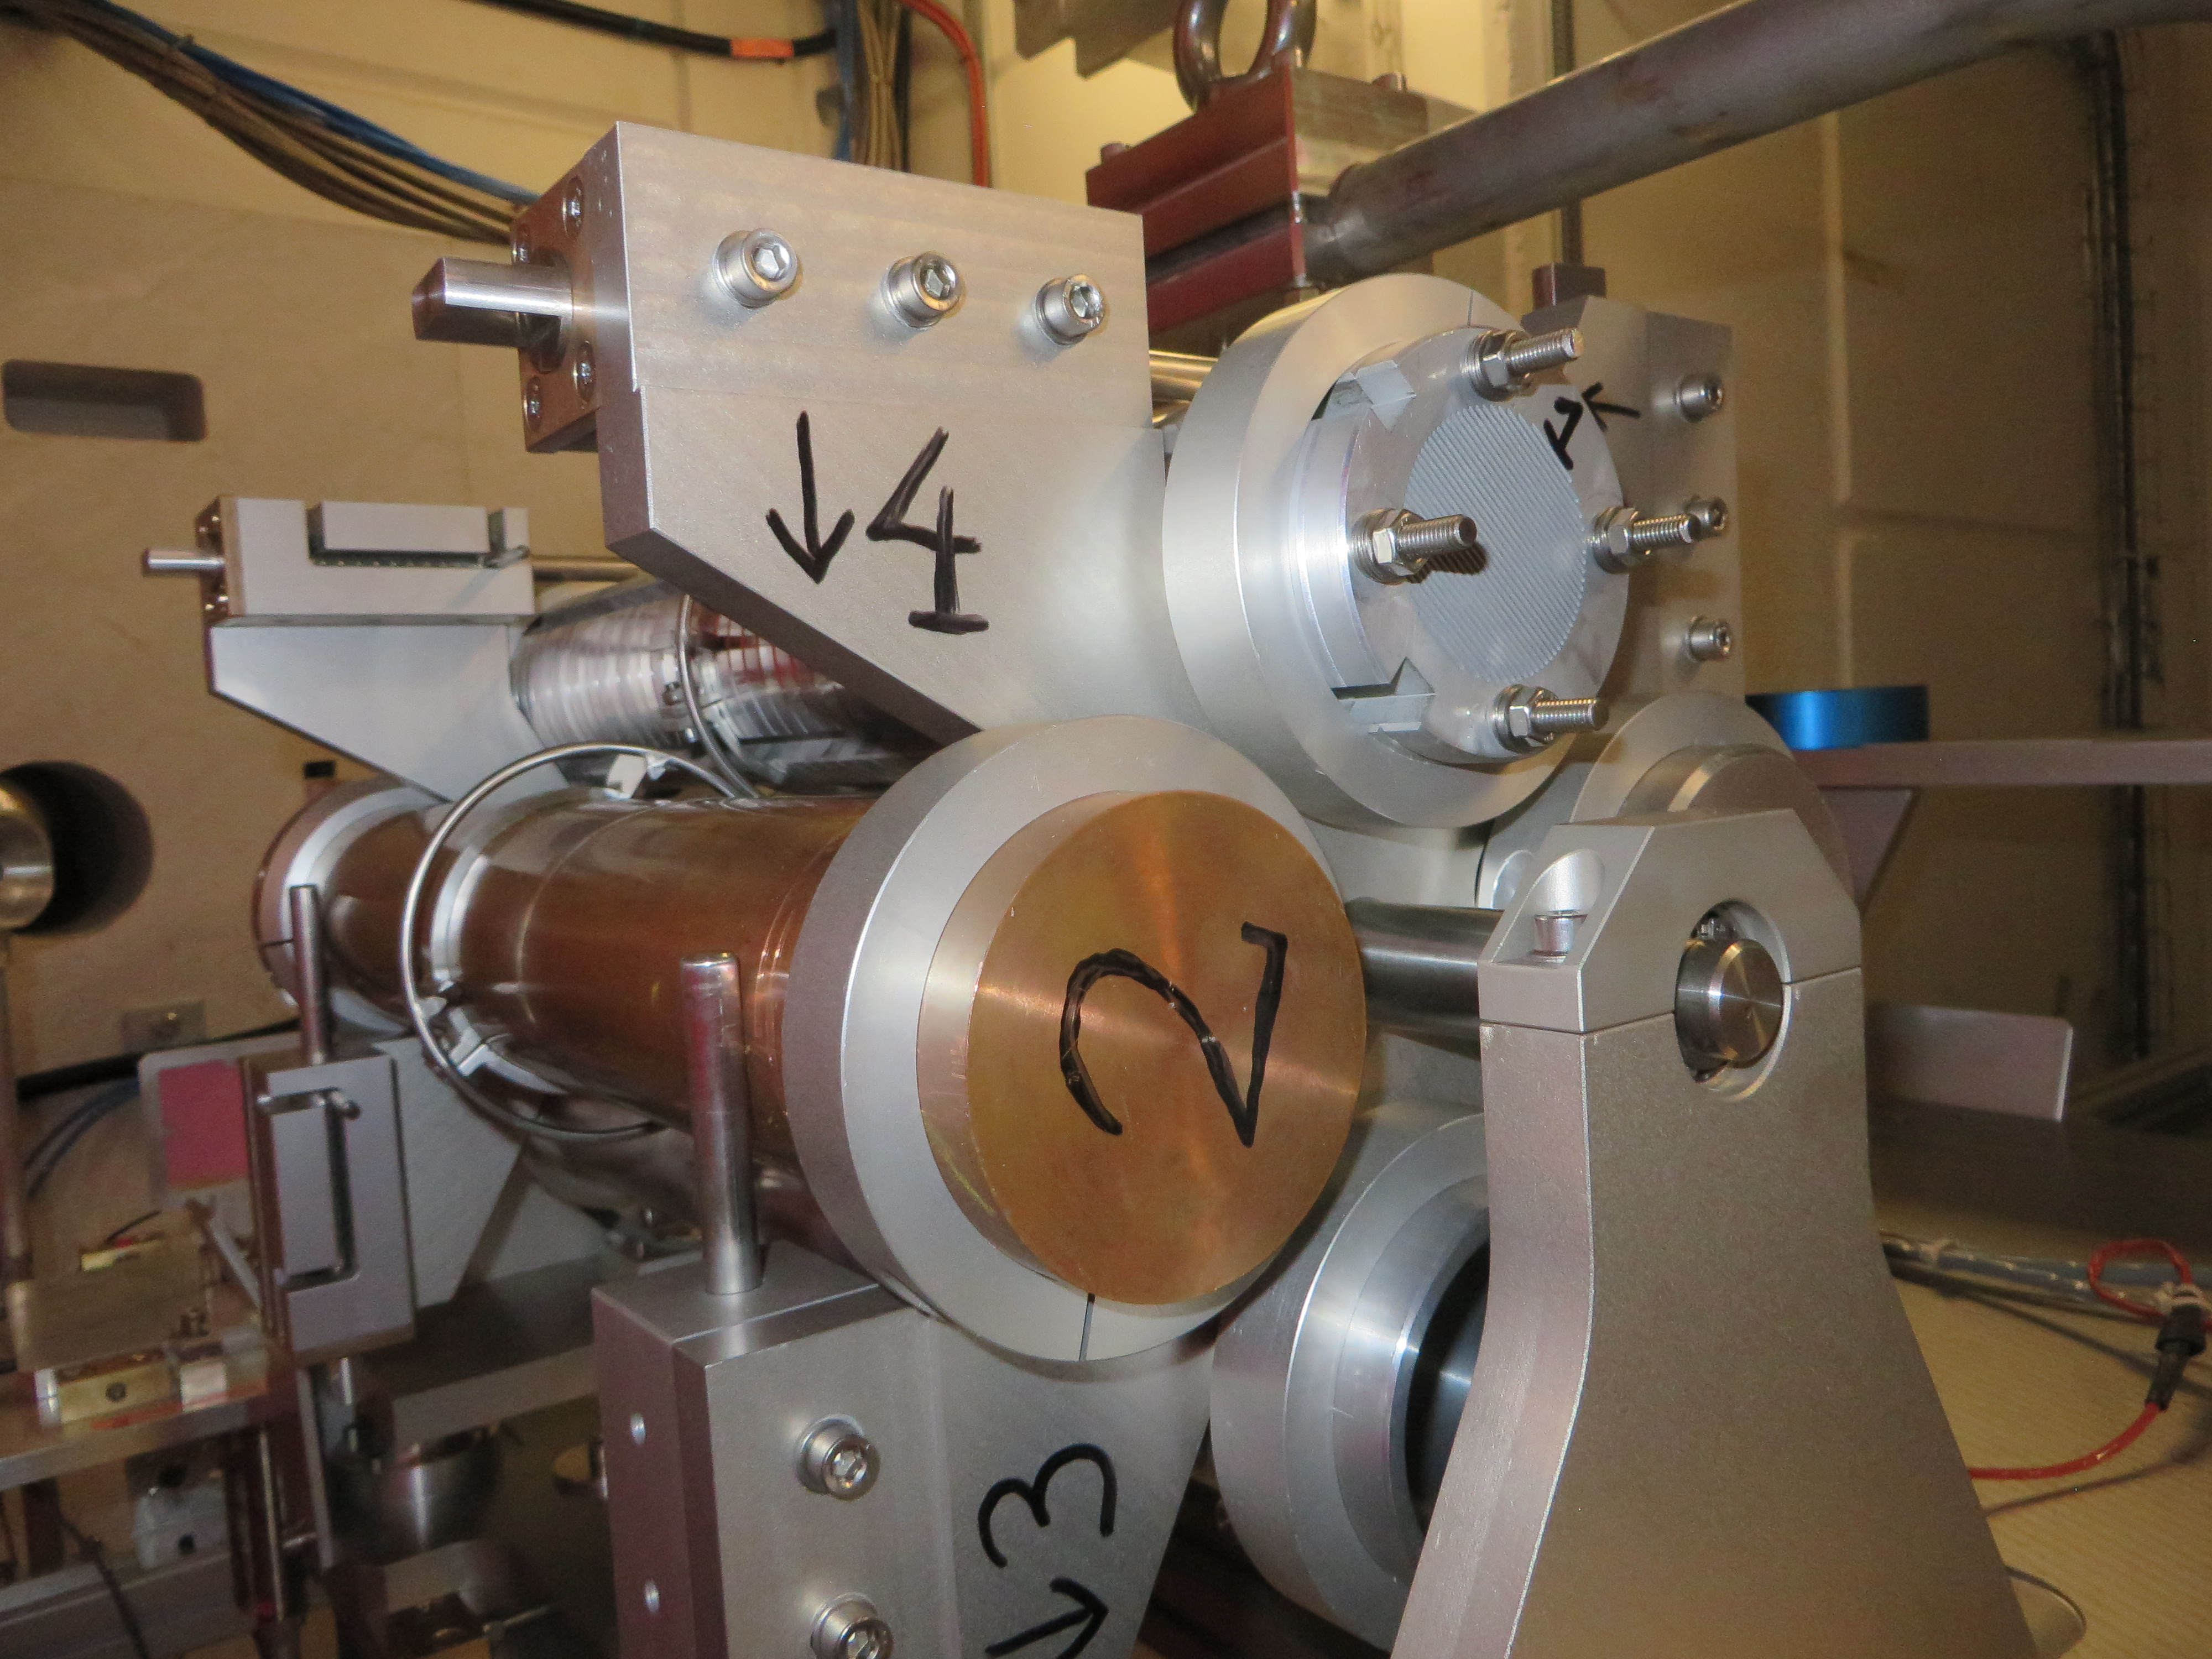
\includegraphics[width=0.9\linewidth]{./images/IMG_1149}
  \caption{A photo of the target table.}
  \label{fig:fluka_target_photo}
\end{subfigure}%
\begin{subfigure}{.5\textwidth}
  \centering
  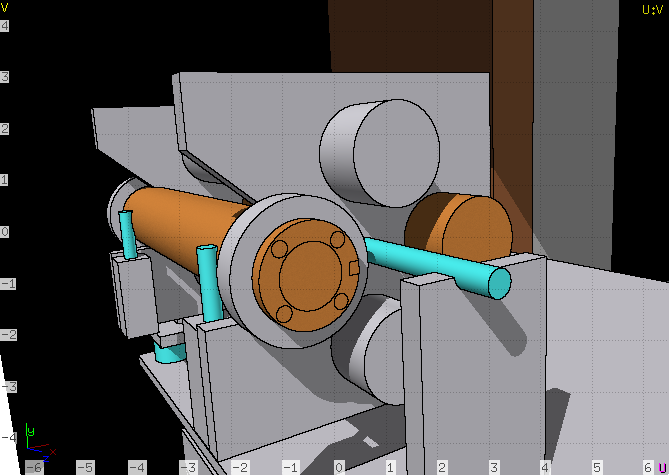
\includegraphics[width=0.9\linewidth]{./images/target_photo_perspective}
  \caption{A screen-shot from the FLUKA geometry}
  \label{fig:fluka_target_geometry}
\end{subfigure}
\caption{A comparison of the real target station and the simplified target station implemented in the FLUKA geometry.}
\label{fig:fluka_target_comparison}
\end{figure}

\subsubsection{FLUKA Physics Configuration}

In FLUKA it is possible to configure the transport of certain particles and likelihood of interactions by changing specific parameters or adding special cards into the input file. The motivation for these is to 'tune' the simulation so that a satisfactory level of accuracy is met, which is usually to do with the statistical uncertainty calculated by the various scoring implemented in the input file, without causing an adverse effect on CPU time. An example of this is the transport threshold for electrons and positrons which can be set to any energy desired. On one hand it's possible to raise the thresholds (or even stop the transport completely) to a level that could even cause non-physical artefacts in the scoring for dose for example, which would reduce the CPU vastly. On the other extreme it's possible to reduce the energy to a level where non-physical effects are very low, but the CPU time per primary particle in the simulation becomes a limiting factor when trying to gain an acceptable level of accuracy in terms of statistics. \\

It was decided to use the NEWDEFA PHYSICS card in the 'defaults' for the CHARM test area calculations with the transport of electrons enabled. This has a 1MeV transport threshold for delta-rays (electrons), which gives a reasonable level of accuracy without greatly impacting the CPU time of the simulation. No biasing was set for the regions inside the test area and no other thresholds were modified. \\

\subsubsection{Scoring}

There are a number of estimators built into FLUKA for calculated various quantities, such as charge particle fluence, dose in air etc. Deciding which estimators to use and how to normalise the data depends on the purpose of the simulation. For the CHARM facility, the focus is on testing of electronics, for which there are a number of appropriate estimators for this purpose. One example is scoring 'high-energy hadrons' i.e. the total flux of hadrons above 20 MeV (deemed the cut-off energy for SEE's in electronics). The selection used for the CHARM FLUKA studies is listed below.

\begin{table}[htbp]
  \sisetup{tight-spacing=true}
  \centering
    \begin{tabular}{l|p{9cm}}
	Estimator & Physical Meaning \\
	\hline
	\hline
	DOSE		& The energy deposited per unit mass \\
	HADGT20M	& Fluence of Hadrons with energy above 20 MeV \\
	SI1MEVNE	& Fluence of 1 MeV (Si) equivalent neutrons \\
	NEUTRON		& Fluence of neutrons \\
	HEHAD-EQ	& Fluence of Hadrons with energy above 20 MeV including intermediate neutrons \\
	THNEU-EQ	& Fluence of thermal-equivalent neutrons \\
    \end{tabular}
	\caption{A table of the estimators used for the CHARM FLUKA calculations. A detailed list can be found in the appendix in table X. More details available in the FLUKA manual.}
	\label{tab:fluka_estimators}
\end{table}
%\documentclass[main.tex]{subfiles}
%\begin{document}

\newpage
\section{FLUKA Results}

Using FLUKA to model the CHARM facility, it is possible to calculate the radiation field at the various test positions with all possible facility configurations: something that would be very difficult and could potentially take months for actual measurements. This chapter attempts to summarise the results for the test positions and Montrac location for a variety of configurations. It goes on to give more detail specifically for the 'cp\_OOOO' configuration as this is a common choice by users of the facility. The tables and information  presented for this configuration are also included for all other configurations in the appendix. \\

From the FLUKA calculations results there are a number different types of information at the test positions. The first of interest is the integral values: dose or particle fluence at that specific location for example. These are useful for simple tests relating to subjects such as tolerance to dose or certain particle types. The second is the fluence of different particles with respect to energy (spectral information) for each of the test positions. This can be used to explore effects correlated with energy, for example the effect of high energy particles on the response of the detector by placing in positions of low and high average particle energy (such as the hardness factor, mentioned in the previous chapter). \\

\subsection{Overview}

\subsubsection*{High-Energy Hadrons}

The fluence of high-energy hadrons for the test positions perpendicular to the target can be reduced by a factor 5 using the half-shielding, and by a factor 10 using the full-shielding, as shown in figure \ref{fig:heh_copper_shielding}. \\

The values for the 1\% (H1), 10\% (H10) and 50\% (H50) hardness factors can be found in tables \ref{tab:hardness1}, \ref{tab:hardness10} and \ref{tab:hardness50} respectively. It is observed that the hardness factor generally increases as the positions move closer to the down-stream positions. This can be explained by the angle with respect to the target, as the secondary particles with a smaller scattering angle will have a higher energy, and those with a large angle will have a lower energy. The hardness factor does not vary highly between targets for the same shielding configuration, and remains almost the same for the positions perpendicular to the beam. The test positions in the beam axis tend to have much higher hardness factors, especially those which are positioned beyond the shielding. \\

The H50 factor is generally very similar between the aluminium targets, and tends to be slightly higher than that for the copper for the same positions and shielding configurations. This may be explained for the test positions down-stream of the target by a lower number of protons interacting with the target due to the lower density, and thus more protons with higher energy reaching the test positions. Overall it is observed that the shielding reduces the hardness factors by a factor 2 for the test positions adjacent to the beam. \\

In terms of HEH spectra, it is possible to emulate many different radiation environments within the CHARM test area. The plot in figure \ref{fig:example_rev_spectra} shows the reverse integral spectra for several radiation environments compared to those at different test positions, marked in grey. A table of the hardness factors for different environments are given in figure \ref{tab:hardness_energies} \cite{radecs2014shortcourse}. A table of acceleration factors for various environments and test configurations at CHARM are shown in \ref{tab:accl_factors_heh}. \\

\newpage

\begin{table}[htbp]
  \centering
    \begin{tabular}{r|l|r|r|r}
    \textbf{Environment} & \textbf{CHARM} & \textbf{Env flux [/y]} & \textbf{CHARM flux [/day]} & \textbf{A factor [y/day]} \\
    \hline
    \hline
    LHC UJ & cp\_CIOO R3 & 2.50E+09 & 2.03E+10 & 8.12 \\
    LHC RR & cp\_OOOO R9 & 1.00E+09 & 6.26E+10 & 62.60 \\
    LHC Tunnel & alh\_OOOO R13 & 6.00E+11 & 1.07E+11 & 0.18 \\
    Ground (NYC) & cp\_CIOO R10 & 1.00E+05 & 1.68E+10 & 1.68E+05 \\
    Atmosphere (20km) & al\_OOOO R11 & 3.80E+07 & 2.68E+11 & 7.05E+03 \\
    Proba II & cp\_CIOO R10 & 2.70E+09 & 1.68E+10 & 6.22 \\
    \end{tabular}%
    \caption{A table of matches for the various radiation environments (based on hardness) with a comparison between the yearly environmental flux and the daily flux at the specific CHARM test position. The 'A' (or acceleration) factor therefore shows the number of years of operation that can be simulated in a single day at CHARM for the respective configuration and test position.}
  \label{tab:accl_factors_heh}%
\end{table}%


\subsubsection*{Dose}
In the CHARM test area is it possible to expose test equipment to a large range of doses, depending on the target, shielding, and test position. The results in table \ref{tab:dose_per_day_all} show the different dose rates possible per day (normal beam conditions) for the different variations of the facility configuration. \\

The lowest doses are observed unsurprisingly with the full shielding and aluminium target (with holes). As this is the least dense target, interaction of the beam with the target is the lowest of the different target options, and therefore the number of secondary particles created with the same number of incoming primary protons is lower. The number of secondary particles can be considered proportional to the dose, however this also depends on the particle type and energy, which will be discussed later in the report. For this facility configuration, the lowest dose is observed at the test positions with the highest angle relative to the beam line, where the fluence of secondaries again would be the lowest. \\

The highest doses are seen at test position 12 (irrespective of shielding, as this position is in line of sight with the target) with the aluminium target with holes. As this target is the least dense, the number of interactions is the lowest of the targets (as stated before). Therefore a large number of primary protons which will directly pass the target with minimal interaction, and therefore with the highest energy and fluence. This would lead to a greater dose deposited on the test equipment. \\

Considering the different shielding configurations, table \ref{tab:dose_per_day_all} generally shows a factor 10 reduction in the dose seen at the shielded test positions between the cases of full shielding and no shielding. The case for half shielding is not shown, however a reduction in dose of around 50\% is observed between full and half shielding cases. \\

The plot in figure \ref{fig:dose_copper_shielding} shows the dose for a slice in the CHARM FLUKA geometry, running from the target towards the entrance wall and highlights the reduction in the dose rate for the different shielding configuration with the copper target. Directly after the shielding a reduction of almost 100 is observed between the cases with and without shielding, which reduces down to a factor of 10 by the test positions around x = 120 cm. \\

\begin{table}[htbp]
\centering
\begin{tabular}{r|c|c|c|c|c|c|c|c|c}
& \multicolumn{3}{c|}{No Shielding} & \multicolumn{3}{c|}{Half Shielding} & \multicolumn{3}{c}{Full Shielding} \\ \cline{2-10}
\textbf{Rack}  & cp    & al    & alh   & cp    & al    & alh & cp    & al    & alh\\ 
\hline
1  &     0.38 &     0.39 &      0.39 &     0.31 &     0.30 &      0.30 &     0.30 &     0.28 &      0.28 \\
2  &     0.41 &     0.43 &      0.43 &     0.32 &     0.30 &      0.30 &     0.32 &     0.29 &      0.29 \\
3  &     0.69 &     0.73 &      0.72 &     0.50 &     0.49 &      0.48 &     0.45 &     0.38 &      0.39 \\
4  &     0.78 &     0.80 &      0.81 &     0.58 &     0.56 &      0.55 &     0.48 &     0.44 &      0.42 \\
5  &     0.89 &     0.92 &      0.92 &     0.64 &     0.62 &      0.61 &     0.50 &     0.45 &      0.47 \\
6  &     0.99 &     1.01 &      1.01 &     0.73 &     0.72 &      0.69 &     0.56 &     0.49 &      0.49 \\
7  &     1.12 &     1.16 &      1.16 &     0.79 &     0.77 &      0.76 &     0.57 &     0.55 &      0.55 \\
8  &     1.23 &     1.26 &      1.27 &     0.88 &     0.85 &      0.83 &     0.63 &     0.61 &      0.61 \\
9  &     1.38 &     1.42 &      1.43 &     0.95 &     0.90 &      0.90 &     0.70 &     0.70 &      0.70 \\
10 &     1.67 &     1.73 &      1.72 &     1.08 &     1.04 &      1.01 &     0.90 &     0.91 &      0.90 \\
11 &    12.57 &    14.34 &     14.63 &    12.47 &    14.24 &     14.57 &    12.48 &    14.26 &     14.57 \\
12 &    24.00 &    24.00 &     24.00 &    24.00 &    24.00 &     24.00 &    24.00 &    24.00 &     24.00 \\
13 &     6.51 &     7.21 &      7.27 &     6.31 &     7.14 &      7.22 &     6.32 &     7.14 &      7.23 \\
\end{tabular}
\caption{A Table of the H1 [GeV] hardness factors for the different target and shielding configurations.}
\label{tab:hardness1}
\end{table}

\begin{table}[htbp]
\centering
\begin{tabular}{r|c|c|c|c|c|c|c|c|c}
& \multicolumn{3}{c|}{No Shielding} & \multicolumn{3}{c|}{Half Shielding} & \multicolumn{3}{c}{Full Shielding} \\ \cline{2-10}
\textbf{Rack}  & cp    & al    & alh   & cp    & al    & alh & cp    & al    & alh\\ 
\hline
1  &     0.18 &     0.19 &      0.19 &     0.16 &     0.15 &      0.15 &     0.16 &     0.15 &      0.15 \\
2  &     0.19 &     0.20 &      0.20 &     0.16 &     0.16 &      0.16 &     0.17 &     0.16 &      0.15 \\
3  &     0.31 &     0.34 &      0.34 &     0.23 &     0.22 &      0.22 &     0.21 &     0.19 &      0.19 \\
4  &     0.36 &     0.39 &      0.39 &     0.25 &     0.24 &      0.24 &     0.22 &     0.20 &      0.19 \\
5  &     0.41 &     0.44 &      0.44 &     0.28 &     0.26 &      0.26 &     0.22 &     0.20 &      0.20 \\
6  &     0.47 &     0.49 &      0.49 &     0.30 &     0.29 &      0.28 &     0.23 &     0.21 &      0.21 \\
7  &     0.51 &     0.56 &      0.56 &     0.32 &     0.30 &      0.30 &     0.23 &     0.22 &      0.22 \\
8  &     0.58 &     0.62 &      0.62 &     0.34 &     0.33 &      0.31 &     0.24 &     0.24 &      0.24 \\
9  &     0.63 &     0.68 &      0.69 &     0.36 &     0.34 &      0.33 &     0.26 &     0.27 &      0.26 \\
10 &     0.78 &     0.85 &      0.85 &     0.39 &     0.38 &      0.38 &     0.33 &     0.34 &      0.33 \\
11 &     6.84 &     8.15 &      8.55 &     6.64 &     8.01 &      8.45 &     6.63 &     8.02 &      8.45 \\
12 &    23.00 &    24.00 &     24.00 &    22.95 &    24.00 &     24.00 &    22.95 &    24.00 &     24.00 \\
13 &     3.35 &     3.87 &      3.90 &     3.21 &     3.81 &      3.85 &     3.22 &     3.81 &      3.85 \\
\end{tabular}
\caption{A Table of the H10 [GeV] hardness factors for the different target and shielding configurations. }
\label{tab:hardness10}%
\end{table}%

\begin{table}[htbp]
\centering
\begin{tabular}{r|c|c|c|c|c|c|c|c|c}
& \multicolumn{3}{c|}{No Shielding} & \multicolumn{3}{c|}{Half Shielding} & \multicolumn{3}{c}{Full Shielding} \\ \cline{2-10}
\textbf{Rack}  & cp    & al    & alh   & cp    & al    & alh & cp    & al    & alh\\ 
\hline
1  &     0.06 &     0.07 &      0.07 &     0.06 &     0.06 &      0.06 &     0.07 &     0.06 &      0.06 \\
2  &     0.06 &     0.07 &      0.07 &     0.06 &     0.06 &      0.06 &     0.07 &     0.06 &      0.06 \\
3  &     0.09 &     0.10 &      0.10 &     0.08 &     0.08 &      0.07 &     0.08 &     0.07 &      0.07 \\
4  &     0.10 &     0.11 &      0.11 &     0.08 &     0.08 &      0.08 &     0.08 &     0.07 &      0.07 \\
5  &     0.11 &     0.12 &      0.12 &     0.09 &     0.08 &      0.08 &     0.07 &     0.07 &      0.07 \\
6  &     0.12 &     0.13 &      0.13 &     0.09 &     0.09 &      0.08 &     0.07 &     0.07 &      0.07 \\
7  &     0.13 &     0.14 &      0.14 &     0.09 &     0.09 &      0.09 &     0.07 &     0.07 &      0.07 \\
8  &     0.14 &     0.16 &      0.15 &     0.09 &     0.09 &      0.09 &     0.07 &     0.07 &      0.07 \\
9  &     0.15 &     0.17 &      0.17 &     0.09 &     0.09 &      0.09 &     0.07 &     0.08 &      0.08 \\
10 &     0.19 &     0.21 &      0.21 &     0.09 &     0.09 &      0.09 &     0.08 &     0.08 &      0.08 \\
11 &     1.79 &     2.69 &      2.87 &     1.57 &     2.56 &      2.76 &     1.57 &     2.55 &      2.76 \\
12 &     7.01 &    20.42 &     21.59 &     6.72 &    20.40 &     21.59 &     6.72 &    20.40 &     21.59 \\
13 &     0.73 &     1.20 &      1.25 &     0.60 &     1.11 &      1.18 &     0.60 &     1.11 &      1.18 \\
\end{tabular}
\caption{A Table of the H50 [GeV] hardness factors for the different target and shielding configurations.}
\label{tab:hardness50}%
\end{table}%

\begin{table}[htbp]
\centering
\begin{tabular}{r|c|c|c|c|c|c}
& \multicolumn{3}{c|}{No Shielding} & \multicolumn{3}{c}{Full Shielding} \\ \cline{2-7}
\textbf{Rack}  & cp    & al    & alh   & cp    & al    & alh\\ 
\hline
1 & 2.48E+16 & 9.41E+15 &  5.46E+15 & 1.52E+15 & 6.89E+14 &  4.64E+14 \\
2 & 2.71E+16 & 1.06E+16 &  6.23E+15 & 1.70E+15 & 8.30E+14 &  5.23E+14 \\
3 & 5.12E+16 & 2.22E+16 &  1.28E+16 & 2.92E+15 & 1.89E+15 &  1.29E+15 \\
4 & 5.15E+16 & 2.34E+16 &  1.34E+16 & 3.18E+15 & 2.51E+15 &  1.53E+15 \\
5 & 4.75E+16 & 2.39E+16 &  1.35E+16 & 3.91E+15 & 3.02E+15 &  1.86E+15 \\
6 & 5.18E+16 & 2.66E+16 &  1.52E+16 & 4.29E+15 & 3.53E+15 &  2.15E+15 \\
7 & 5.09E+16 & 2.74E+16 &  1.58E+16 & 4.56E+15 & 4.29E+15 &  2.70E+15 \\
8 & 4.85E+16 & 2.82E+16 &  1.62E+16 & 5.38E+15 & 5.14E+15 &  3.28E+15 \\
9 & 4.65E+16 & 2.90E+16 &  1.66E+16 & 6.15E+15 & 6.35E+15 &  3.86E+15 \\
10 & 5.41E+16 & 3.89E+16 &  2.23E+16 & 8.91E+15 & 1.02E+16 &  6.26E+15 \\
11 & 1.21E+17 & 3.79E+17 &  2.56E+17 & 1.19E+17 & 3.86E+17 &  2.60E+17 \\
12 & 2.36E+17 & 1.08E+18 &  1.26E+18 & 2.39E+17 & 1.08E+18 &  1.26E+18 \\
13 & 1.01E+17 & 2.30E+17 &  1.34E+17 & 1.06E+17 & 2.34E+17 &  1.36E+17 \\
\end{tabular}
\caption{A Table of dose (Gy) per day for the different target and shielding configurations. }
\label{tab:dose_per_day_all}%
\end{table}%

\begin{figure}[ht!]
	\centering
	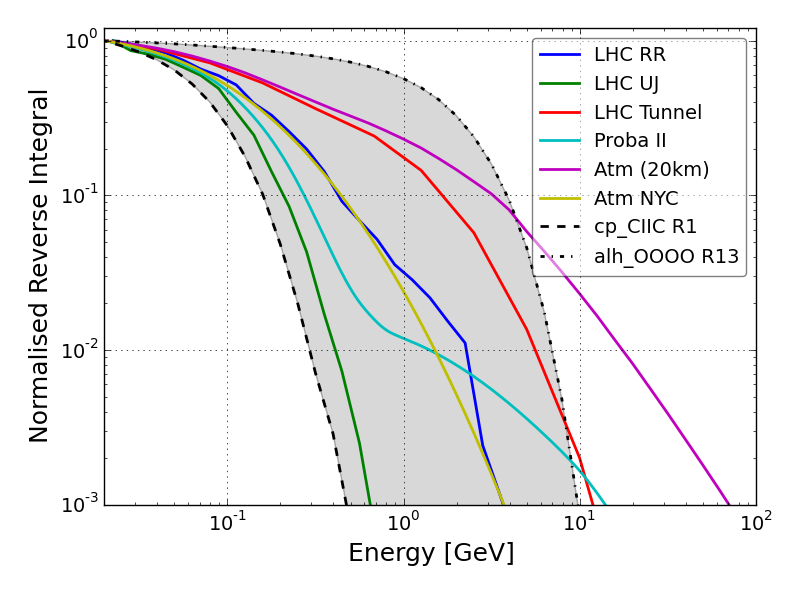
\includegraphics[width=0.7\textwidth]{./images/hardness/all_env_charm}
	\caption{A plot of the reverse integral spectra for test positions at CHARM (in grey), compared with different radiation environments, normalised to 20 MeV.}
	\label{fig:example_rev_spectra}
\end{figure}

\begin{figure}[ht!]
	\centering
	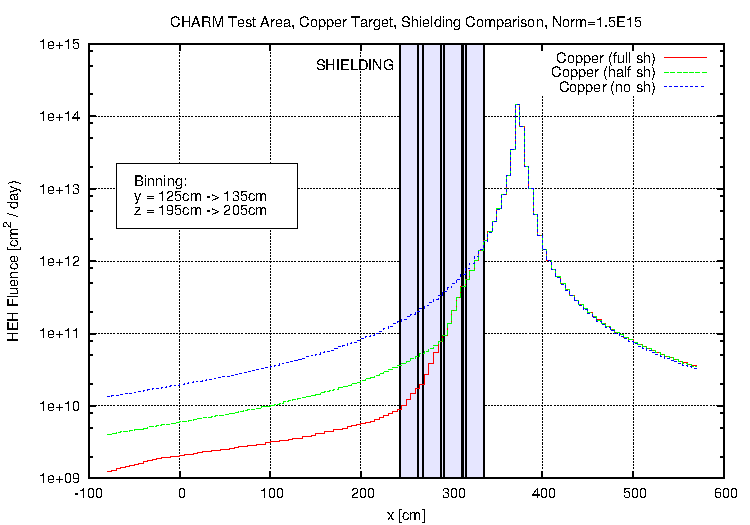
\includegraphics[scale=1.1]{./images/heh_comparison_with_shielding}
	\caption{A plot of the HEH fluence for a slice in the test area geometry from the target, towards the entrance. It shows that with the shielding, there is a reduction in the HEH fluence of a factor 10.}
	\label{fig:HEH_copper_shielding}
\end{figure}

\begin{figure}[ht!]
	\centering
	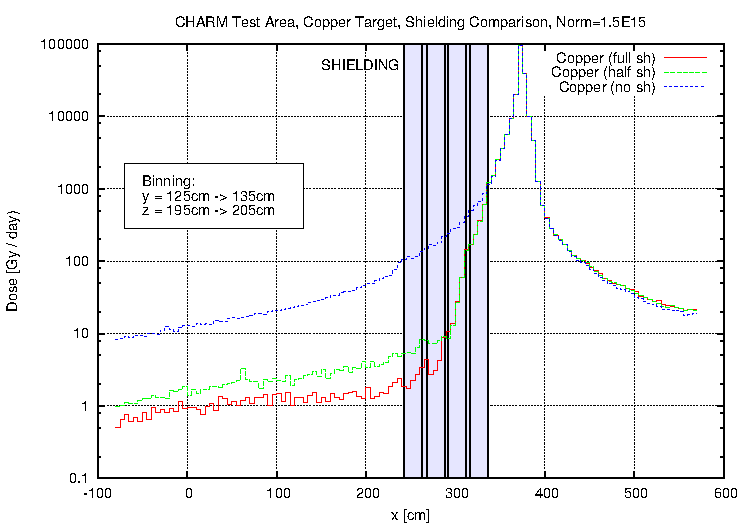
\includegraphics[scale=1.1]{./images/dose_comparison_with_shielding}
	\caption{A plot of the dose for a slice in the test area geometry from the target, towards the entrance. The shielding reduces the dose by almost a factor 100 close to the shielding, and reduces down to a factor 10 by the test positions.}
	\label{fig:dose_copper_shielding}
\end{figure}

\clearpage

\begin{figure}[ht!]
	\centering
	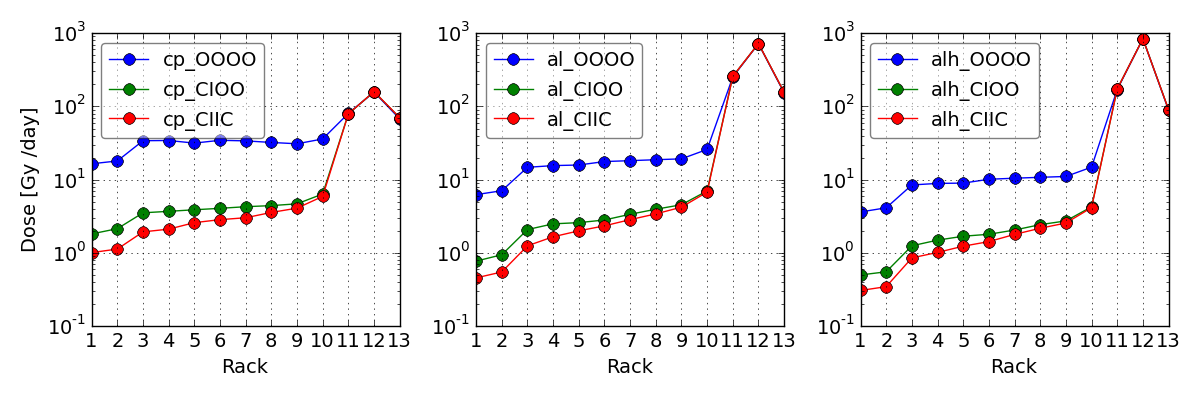
\includegraphics[width=\textwidth]{./images/test_positions/dose_per_day}
	\caption{A plot of the dose per day at the different test positions with the different facility configurations.}
	\label{fig:dose_test_pos}
\end{figure}

\begin{figure}[ht!]
	\centering
	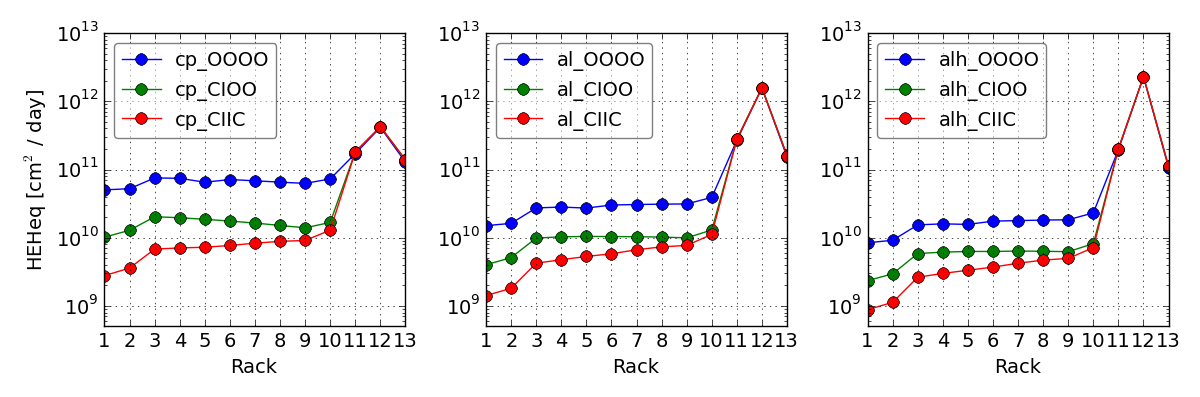
\includegraphics[width=\textwidth]{./images/test_positions/heheq_per_day}
	\caption{A plot of the high energy hadron fluence per day at the different test positions with the different facility configurations.}
	\label{fig:dose_test_pos}
\end{figure}

\clearpage

\subsection{Hardness Factors}

The hardness factors for each test position and configuration have been calculated using the reverse integral of the HEH fluence (see previous chapter for more details on the hardness factors). The same values have also been calculated from data-sets measured (and in some cases simulated) of real environments ranging from accelerator alcove areas where control electronics may be placed, to upper atmospheric and space environments where for example electronics on satellites are exposed to mixed-field radiation environments much harsher than those found at ground level. These two sources of information have been compared in order to find the places at CHARM to test electronics in the same environments they would be used in. This would then give the best indication of their sensitivity (or tolerance) to radiation by exposing them to radiation fields as similar as possible to their intended application. \\

The method to choose the best match is based on trying to find the test positions at CHARM that have the same hardness factors as the desired mixed-field. This is achieved by finding the hardness factors for the desired field, and calculating the difference for each possible test position and configuration at CHARM. The resulting data-table is then sorted to minimise the difference between the value for each hardness factor. Depending on the application, the best match can change. An example of this is when trying to find a test position which is exposed to particle energies of the same magnitude as the desired mixed-field, where there may be a compromise between matching the high energy of the field, and getting correct proportion of lower energy particles. This will depend on the test device and it's error rate as a function of energy. \\

For radiation environments around the HEH LHC, as number of matches have been found. A plot of the reverse integral spectra for a number of simulated LHC environments are shown in figure \ref{fig:lhc_charm_comparison}. These radiation fields could be considered as typical accelerator mixed-field environments, where the UJ and RR areas correspond to shielded areas near the beam-line, and the tunnel area as an un-shielded environment exposed to high energy particle showers from direct beam losses on the beam-line elements. \\

% Reference for data, elias simulations. Table of hardness factors and CHARM matches. Use the ipython notebook to get the hardness factors for the specific cases. Hopefully they match the table in the previous chapter. If not, which should we use??

\begin{table}[htbp]
\centering
\begin{tabular}{l|c|l|l|l}
\textbf{Environment} & \textbf{HEH /cm$^{2}$/ y} & \multicolumn{3}{c}{\textbf{Hardness Factor}} \\ \cline{3-5}
				& & H50   & H10   & H1 \\
\hline
\hline
Proba II (800km, 98$^{o}$)		& 2.7E+09 & 0.094 & 0.273 & 1.406 \\
Atm (20km)						& 3.8E+07 & 0.20  & 3.242 & 17.814 \\
Ground (NYC)					& 1.0E+05 & 0.103 & 0.442 & 1.506 \\
LHC UJ							& 2.5E+09 & 0.087 & 0.212 & 0.421 \\
LHC RR							& 1.0E+09 & 0.116 & 0.431 & 2.312 \\
LHC Tunnel						& 6.0E+11 & 0.19  & 1.901 & 6.56 \\
\end{tabular}%
\caption{A table of hardness factors for the reference spectra used for comparisons with the CHARM test positions. The hardness factors are in units of GeV.}
\label{tab:hardness_factor_references}%
\end{table}%

\newpage

\begin{figure}[ht!]
	\centering
	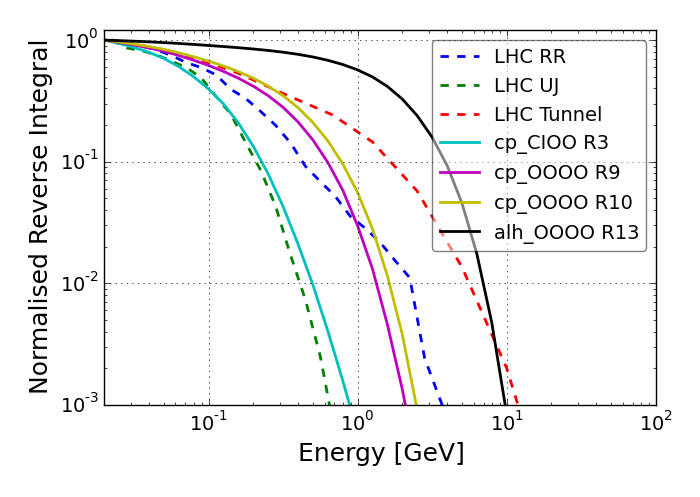
\includegraphics[width=0.7\textwidth]{./images/hardness/lhc_charm_comparison}
	\caption{A plot of several reverse integral spectra from simulations of LHC environments, along with matching CHARM test configurations.}
	\label{fig:lhc_charm_comparison}
\end{figure}

\begin{table}[htbp]
\centering
\begin{tabular}{l|l|l|l}
\textbf{environment} & \multicolumn{3}{c}{\textbf{Hardness Factor}} \\ \cline{2-4}
				& H50   & H10   & H1 \\
\hline
\hline
\rowcolor{gray!30} LHC UJ & 0.087 & 0.212 & 0.421 \\
cp\_CIOO R3	& 0.079 & 0.232 & 0.498 \\

\hline
\rowcolor{gray!30} LHC RR & 0.116 & 0.431 & 2.312 \\
cp\_OOOO R9  & 0.152 & 0.628 & 1.378 \\
cp\_OOOO R10 & 0.190 & 0.782 & 1.665 \\

\hline
\rowcolor{gray!30} LHC Tunnel & 0.19  & 1.901 & 6.56 \\
alh\_OOOO R13 & 1.249 & 3.898 & 7.273 \\
\end{tabular}%
\caption{}
\label{tab:hardness_factor_lhc}%
\end{table}%

\clearpage

\begin{figure}[ht!]
	\centering
	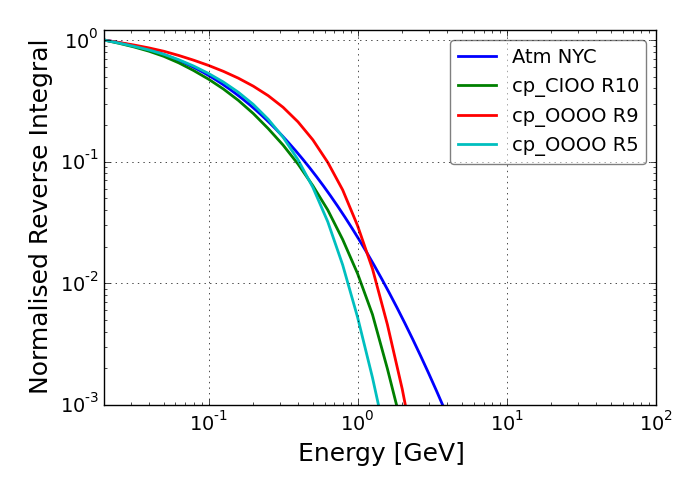
\includegraphics[width=0.7\textwidth]{./images/hardness/atm0km_charm_comparison}
	\caption{A plot of the reverse integral HEH spectrum at ground level (New York, Jedec89 Standard), with a number of CHARM test configurations with close matches.}
	\label{fig:atm0km_charm_comparison}
\end{figure}

\begin{table}[htbp]
\centering
\begin{tabular}{l|l|l|l}
\textbf{environment} & \multicolumn{3}{c}{\textbf{Hardness Factor}} \\ \cline{2-4}
				& H50   & H10   & H1 \\
\hline
\hline
\rowcolor{gray!30} Ground (NYC) & 0.103 & 0.442 & 1.506 \\
cp\_CIOO R10	& 0.094 & 0.389 & 1.080 \\
cp\_OOOO R9		& 0.152 & 0.628 & 1.378 \\
cp\_OOOO R5 	& 0.110 & 0.407 & 0.890 \\
\end{tabular}%
\caption{}
\label{tab:hardness_factor_atm_nyc}%
\end{table}%

\clearpage

\begin{figure}[ht!]
	\centering
	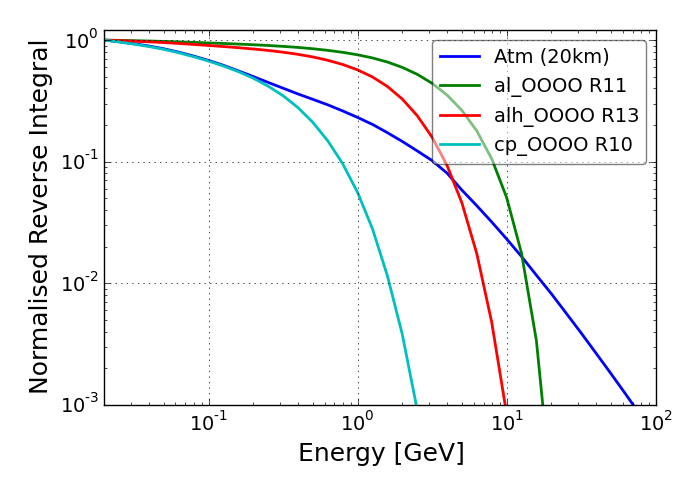
\includegraphics[width=0.7\textwidth]{./images/hardness/atm20km_charm_comparison}
	\caption{A plot of the reverse integral HEH spectrum at an altitude of 20km (Geneva, Switzerland), with a number of CHARM test configurations with close matches. The atmospheric HEH spectra extends to energies beyond those achievable at CHARM, however the intermittent hardness energies can be matched.}
	\label{fig:atm20km_charm_comparison}
\end{figure}

\begin{table}[htbp]
\centering
\begin{tabular}{l|l|l|l}
\textbf{environment} & \multicolumn{3}{c}{\textbf{Hardness Factor}} \\ \cline{2-4}
				& H50   & H10   & H1 \\
\hline
\hline
\rowcolor{gray!30} Atm (20km) & 0.200 & 3.242 & 17.814 \\
al\_OOOO R11	& 2.695 & 8.153 & 14.337 \\
alh\_OOOO R13	& 1.249 & 3.898 & 7.273 \\
cp\_OOOO R10 	& 0.190 & 0.782 & 1.665 \\
\end{tabular}%
\caption{}
\label{tab:hardness_factor_atm_nyc}%
\end{table}%

\clearpage

\begin{figure}[ht!]
	\centering
	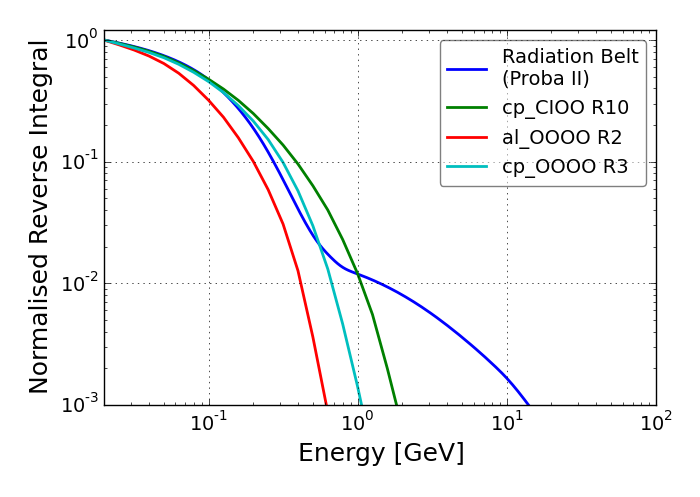
\includegraphics[width=0.7\textwidth]{./images/hardness/space_charm_comparison}
	\caption{A plot of the reverse integral HEH spectrum for the proton belt (Proba II orbit), with a number of CHARM test configurations with close matches.}
	\label{fig:space_charm_comparison}
\end{figure}

\begin{table}[htbp]
\centering
\begin{tabular}{l|l|l|l}
\textbf{environment} & \multicolumn{3}{c}{\textbf{Hardness Factor}} \\ \cline{2-4}
				& H50   & H10   & H1 \\
\hline
\hline
\rowcolor{gray!30} Proba II & 0.094 & 0.273 & 1.406 \\
cp\_CIOO R10	& 0.094 & 0.389 & 1.080 \\
al\_OOOO R2		& 0.068 & 0.200 & 0.428 \\
cp\_OOOO R3 	& 0.090 & 0.314 & 0.691 \\
\end{tabular}%
\caption{}
\label{tab:hardness_factor_proba}%
\end{table}%

\clearpage

\subsection{Copper Target without Shielding}

The following results chapter focuses on the analysis of the calculations using the copper target configuration without shielding (\textbf{cp\_OOOO}). The same tables and plots for the other facility configurations can be found in the appendix. All results tables can also be found at \url{http://thornton.web.HEH.ch/}  \\

The data for all test positions in the cp\_OOOO configuration are shown in table \ref{tab:cpOOOO-alldata}. The results include dose and HEH fluence rates per day (normalised for 1.5E15 protons), spectra content as a percentage of the total HEH fluence, 'R' factors and hardness factors. \\

An example plot of the spectra seen at a test location is shown in figure \ref{fig:cpOOOO_spectra}. the plot shows the relative fluences (arbitrary values) for a range of different particles. Of particular interest is the neutron spectrum which typically has a much larger energy range than the other particles, and is strongly influenced by the shielding and position of the test device. \\

The dose and HEH fluence varies largely depending on the position within the test area, and this is shown in figures \ref{fig:cpOOOO_dosemap} and \ref{fig:cpOOOO_HEHmap}. The plots show the dose and HEH fluence mapped out at the beam height for the whole test area. Large gradients can be seen at the test positions close to the beam axis, therefore testing in these positions should be analysed and set-up carefully, ideally with small test equipment to minimise the variation within the device. Some 'shadows' can be seen in the HEH fluence due to the interaction with the shielding support beams. This is true for all targets, but has less of an impact when using the shielding. \\

\begin{table}[htbp]
\centering
\begin{tabular}{c|P{1.7cm}|P{1.7cm}|c|c|c|c|c|c|c|c}
\textbf{Rack} & \textbf{Dose Gy/ day} & \textbf{HEH /cm$^{2}$/ day} & \multicolumn{4}{c|}{\textbf{Composition}} & \textbf{R} & 				\multicolumn{3}{c}{\textbf{Hardness energy}} \\ \cline{4-7} \cline{9-11}  
& & & n & p & $\pi^{\pm}$ & k & & H50 & H10 & H1 \\
\hline
\hline
1	&	1.65E+01	&	5.03E+10	&	82.90	&	7.04	&	9.54	&	0.20	&	3.48	&	0.06	&	0.18	&	0.38	\\
2	&	1.81E+01	&	5.23E+10	&	82.50	&	7.08	&	9.80	&	0.23	&	3.15	&	0.06	&	0.19	&	0.41	\\
3	&	3.41E+01	&	7.53E+10	&	72.40	&	13.00	&	14.00	&	0.44	&	2.05	&	0.09	&	0.31	&	0.69	\\
4	&	3.43E+01	&	7.44E+10	&	70.30	&	13.70	&	15.30	&	0.49	&	2.06	&	0.10	&	0.36	&	0.78	\\
5	&	3.16E+01	&	6.52E+10	&	69.80	&	13.80	&	15.70	&	0.57	&	2.37	&	0.11	&	0.41	&	0.89	\\
6	&	3.46E+01	&	7.13E+10	&	66.40	&	15.60	&	17.10	&	0.62	&	2.19	&	0.12	&	0.47	&	0.99	\\
7	&	3.39E+01	&	6.84E+10	&	64.90	&	16.10	&	18.10	&	0.70	&	2.30	&	0.13	&	0.51	&	1.12	\\
8	&	3.23E+01	&	6.53E+10	&	63.20	&	16.70	&	19.20	&	0.74	&	2.39	&	0.14	&	0.58	&	1.23	\\
9	&	3.10E+01	&	6.26E+10	&	62.30	&	16.80	&	19.90	&	0.83	&	2.51	&	0.15	&	0.63	&	1.38	\\
10	&	3.61E+01	&	7.28E+10	&	58.80	&	17.20	&	22.70	&	1.11	&	2.05	&	0.19	&	0.78	&	1.67	\\
11	&	8.04E+01	&	1.71E+11	&	34.50	&	23.50	&	37.70	&	4.06	&	0.74	&	1.79	&	6.84	&	12.60	\\
12	&	1.57E+02	&	4.15E+11	&	24.50	&	49.10	&	23.60	&	2.60	&	0.30	&	7.01	&	23.00	&	24.00	\\
13	&	6.77E+01	&	1.28E+11	&	41.30	&	19.50	&	35.60	&	3.41	&	1.03	&	0.73	&	3.35	&	6.51	\\
\end{tabular}
\caption{A table of the spectra content and hardness factors for the test area configuration with copper target and without shielding.}
\label{tab:cpOOOO-alldata}%
\end{table}%


\begin{figure}[!ht]
	\centering
	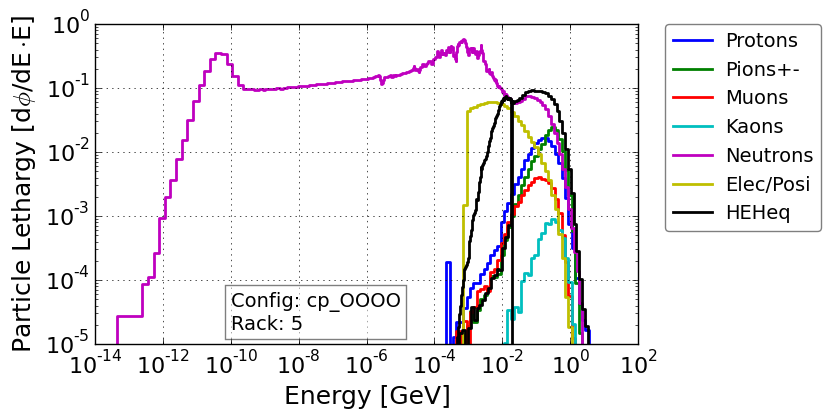
\includegraphics[scale=0.6]{./images/spectra_cp_OOOO_r5}
	\caption{An example plot of the radiation spectra at a test position for the facility configuration with the the copper target without shielding.}
	\label{fig:cpOOOO_spectra}
\end{figure}

\begin{figure}[!ht]
	\centering
	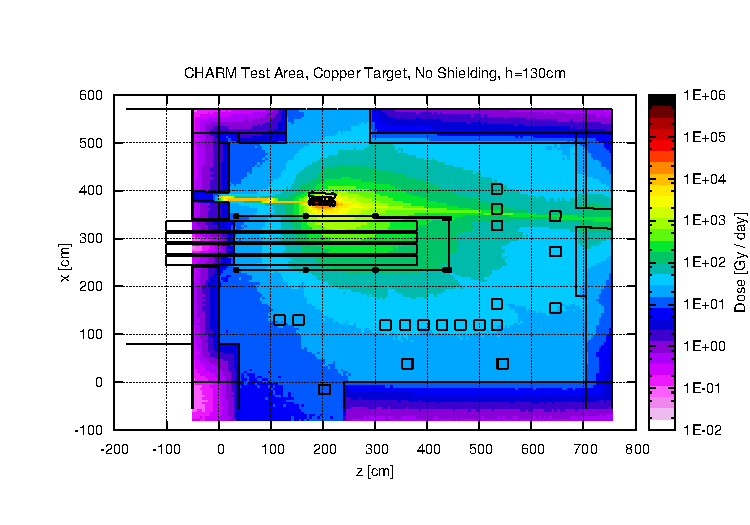
\includegraphics[width=\textwidth]{./images/dose_test_area_cpOOOO}
	\caption{A plot of the dose normalised per day inside the test area at beam height (1.5E15 protons per day).}
	\label{fig:cpOOOO_dosemap}
\end{figure}

\begin{figure}[!ht]
	\centering
	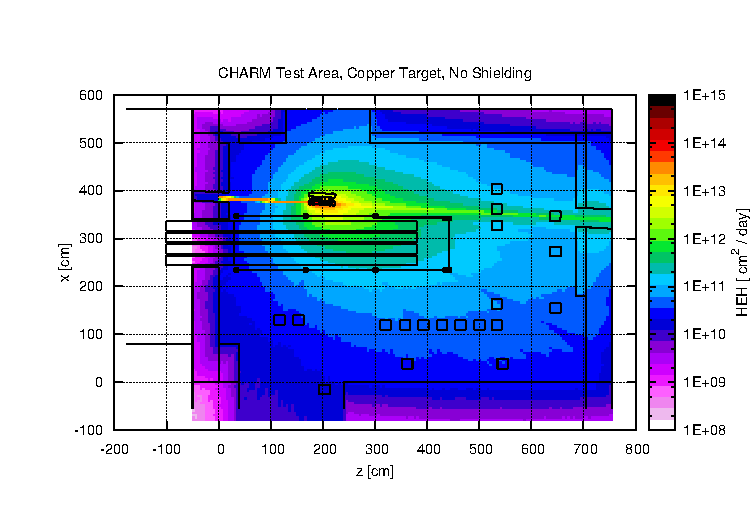
\includegraphics[width=\textwidth]{./images/heh_test_area_cpOOOO}
	\caption{A plot of the HEH fluence normalised per day inside the test area at beam height (1.5E15 protons per day).}
	\label{fig:cpOOOO_HEHmap}
\end{figure}

\clearpage
\subsection{Uncertainties}

There are a number of errors and uncertainties associated with the FLUKA calculations. The first main contributing factor is the accuracy of the geometry. This is in term of position of objects inside the main simulation geometry, materials and dimensions. Secondly there may be errors when comparing the calculations to tests made in the real facility due to positioning, and accurately the device was placed. There needs to be considerations for the test device itself, as the size of the sensitive volume may be large. These points are explored below with the aim of summarizing the various potential errors. \\

The geometry for the CHARM FLUKA calculations was built using the Flair tool \cite{FLAIR1}. Initially it was based on the technical drawings produced for the construction of the facility, however once built it was possible to re-check the dimensions and verify that the drawings were correct. There were some small differences between the drawings and actual construction (for example the back wall build 1m further from the target than initially planned), however these were corrected for the final FLUKA geometry. The bodies in the geometry can be generally considered to be accurate within 1-2cm, with smaller objects such as the target, accurate within 1cm. \\

The accuracy of the test positions within the test facility was also verified during tests of the conveyor system, and can be considered accurate within 1-2cm in each axis. Another error to consider at the test positions is related to the gradients of the radiation, i.e. in positions close to the beam axis, the radiation field can very up to 1\% per centimetre. Therefore the physical size of the test equipment needs to be considered when choosing the test position with the facility. \\

A more detailed analysis of the errors and gradients in the test positions will follow. \\
%\documentclass[main.tex]{subfiles}
%\begin{document}

\newpage
\section{Measurements and Testing}
This chapter will summarise a number of measurements performed at CHARM, with the aim of later benchmarking the FLUKA calculated data, so that in the future we can rely confidently on the calculations, and minimise the number of measurements needed. There are a number of key areas of interest for the measurements which can be divided into the following; non-shielded test-area positions, shielded test-area positions, and the in-beam Montrac position \cite{charmblown} \\

A series of measurements were performed during 2014 and 2015 \cite{charmcalibration} using the Radmon \cite{Wijnands_radmon} detector system for dose and high-energy hadron equivalent fluence at a number of different test positions and facility configurations. A comparison has been made for the integral dose and fluence values calculated using FLUKA for respective positions, and the results for which are shown in tables \ref{tab:datatable-cpOOOO-dose}, \ref{tab:datatable-cpOOOO-heheq}, \ref{tab:datatable-cpCIIC-dose} and \ref{tab:datatable-cpCIIC-heheq}, where M/F stands for measurement divided by the value calculated with FLUKA. All the Radmon dose and HEHeq data was normalised per proton on target using the SEC1 with the calibration factor of 1.84E7 protons per count (or 554242 SEC1 counts) which based on aluminium foil activation \cite{pozzi2015}. The errors on the Radmon measurements can be assumed around 20\%. All values are an average of 3 measurements taken over 3 different test periods. \\

There is a systematic overestimate of the dose for both shielding configurations. This has been found to be due to the difference between scoring in air in the calculations compared to measuring the dose in silicon using the Radmon. Another contribution to the difference has been found in which thresholds are used when scoring the dose in air or silicon. As the thresholds are lowered, the dose scored in FLUKA reduces and becomes much more compatible with the measurements. A more detailed study on this is currently being made \cite{matteo2016}. \\

In the case without shielding. the calculations seem able to accurately model the high-energy hadron equivalent fluence, with the ratio between measurement and calculations around 1 in table \ref{tab:datatable-cpOOOO-heheq}. One exception to this is at position 10, however this value is based on only 2 measurements. For the case with shielding, the match is less strong, showing around a 20\% overestimate of the calculations. This may be due to a difference in the way the high-energy hadron equivalent fluence is modelled in FLUKA, as the measurements were made using the V6 Radmon and the original implementation was based on the V5 Radmon system. This has a particular impact on the 'intermediate' energy neutrons, for which there is a significantly different response between the 2 detectors. \\

\begin{table}[htbp]
  \centering
    \begin{tabular}{c|r|r|r}
    \textbf{Position} & \textbf{Radmon} & \textbf{FLUKA} & \textbf{M/F} \\
    \hline
    \hline
    1     & 6.35E-15 & 1.10E-14 & 0.69 \\
    2     & 6.85E-15 & 1.21E-14 & 0.68 \\
    3     & 1.26E-14 & 2.28E-14 & 0.66 \\
    5     & 9.26E-15 & 2.11E-14 & 0.53 \\
    7     & 1.18E-14 & 2.26E-14 & 0.63 \\
    9     & 1.11E-14 & 2.07E-14 & 0.64 \\
    10    & 1.36E-14 & 2.40E-14 & 0.68 \\
    \end{tabular}%
    \caption{A table of dose measurements showing the comparison with the FLUKA calculations at various test positions for the copper target (no shielding) configuration. The units for the dose are given in Gy per primary particle. }
  \label{tab:datatable-cpOOOO-dose}%
\end{table}%

\begin{table}[htbp]
  \centering
    \begin{tabular}{c|r|r|r}
    \textbf{Position} & \textbf{Radmon} & \textbf{FLUKA} & \textbf{M/F} \\
    \hline
    \hline
    1     & 2.70E-05 & 3.35E-05 & 0.97 \\
    2     & 2.30E-05 & 3.49E-05 & 0.79 \\
    3     & 4.02E-05 & 5.02E-05 & 0.96 \\
    5     & 3.62E-05 & 4.34E-05 & 1.00 \\
    7     & 3.92E-05 & 4.56E-05 & 1.03 \\
    9     & 3.70E-05 & 4.17E-05 & 1.06 \\
    10    & 5.69E-05 & 4.86E-05 & 1.41 \\
    \end{tabular}%
    \caption{A table of HEHeq measurements showing the comparison with the FLUKA calculations at various test positions for the copper target (no shielding) configuration. The units of HEHeq are given per centimetre squared, per primary particle. }
  \label{tab:datatable-cpOOOO-heheq}%
\end{table}%

\begin{table}[htbp]
  \centering
    \begin{tabular}{c|r|r|r}
    \textbf{Position} & \textbf{Radmon} & \textbf{FLUKA} & \textbf{M/F} \\
    \hline
    \hline
    1     & 4.67E-16 & 6.78E-16 & 0.83 \\
    2     & 4.82E-16 & 7.57E-16 & 0.76 \\
    3     & 7.60E-16 & 1.30E-15 & 0.70 \\
    5     & 1.00E-15 & 1.74E-15 & 0.69 \\
    7     & 1.18E-15 & 2.03E-15 & 0.70 \\
    9     & 1.18E-15 & 2.74E-15 & 0.52 \\
    \end{tabular}%
    \caption{A table of dose measurements showing the comparison with the FLUKA calculations at various test positions for the copper target (full shielding) configuration. The units for the dose are given in Gy per primary particle. }
  \label{tab:datatable-cpCIIC-dose}%
\end{table}%

\begin{table}[htbp]
  \centering
    \begin{tabular}{c|r|r|r}
    \textbf{Position} & \textbf{Radmon} & \textbf{FLUKA} & \textbf{M/F} \\
    \hline
    \hline
    1     & 1.34E-06 & 1.86E-06 & 0.87 \\
    2     & 1.51E-06 & 2.39E-06 & 0.76 \\
    3     & 2.74E-06 & 4.54E-06 & 0.72 \\
    5     & 2.94E-06 & 5.13E-06 & 0.69 \\
    7     & 3.45E-06 & 5.55E-06 & 0.75 \\
    9     & 4.36E-06 & 6.08E-06 & 0.86 \\
    \end{tabular}%
    \caption{A table of HEHeq measurements showing the comparison with the FLUKA calculations at various test positions for the copper target (full shielding) configuration. The units of HEHeq are given per centimetre squared, per primary particle.}
  \label{tab:datatable-cpCIIC-heheq}%
\end{table}%
\section{Summary}

The CHARM facility hosted on the T8 beam-line has been running since the autumn of 2014 and has since begun testing with users. There are a number of different configurations possible within the test area enabling testing of electronics in mixed-field radiation emulating many different known radiation environments (including atmosphere, space and accelerator alcoves). During the early commissioning period, each facility configuration was tested and the typical beam conditions for each have been described in the facility description chapter. \\

Using the FLUKA Monte Carlo code, calculations have been performed to describe the radiation field, ranging from the spectra at the different test locations, to dose and particles fluences in and around the target. Following a number of measurements in the test area using the Radmon system, an initial analysis has been started to compare the measured values against those calculated using FLUKA. The first analysis shows a poor match with respect to dose where the calculations can be up to a factor 2 higher than the measurements. However the measurements are very close with the calculations for the high-energy hadrons across the various test positions. The analysis so far is limited to configurations with the copper target, however more datasets are available for future analysis. \\

A more detailed analysis will follow to address the discrepancy for the dose calculations. Additional work is focusing on verifying the hardness factors with a series of measurements made in 2015 using an experimental SRAM based detector. \\

\bibliographystyle{plain}
\bibliography{./references}

\appendix
%\documentclass[main.tex]{subfiles}
%\begin{document}

\section{Appendix}
\subsection{Facility Information}

% Table generated by Excel2LaTeX from sheet 'Sheet1'
\begin{table}[htbp]
  \centering
    \begin{tabular}{r|c|c|c}
    \textbf{Position} & \textbf{x [cm]} & \textbf{y [cm]} & \textbf{z [cm]} \\
    \hline
    \hline
    1     & 130   & 129   & 117 \\
    2     & 130   & 129   & 153 \\
    3     & 120   & 129   & 320 \\
    4     & 120   & 129   & 358 \\
    5     & 120   & 129   & 393 \\
    6     & 120   & 129   & 429 \\
    7     & 120   & 129   & 464 \\
    8     & 120   & 129   & 501 \\
    9     & 120   & 129   & 534 \\
    10    & 163   & 129   & 534 \\
    11    & 327   & 129   & 534 \\
    12    & 362   & 129   & 534 \\
    13    & 403   & 129   & 534 \\
    \end{tabular}%
    \label{tab:charm_test_pos}
    \caption{A table of the test position coordinates in the CHARM test area, relative to the FLUKA geometry.}
  \label{tab:test_positions}%
\end{table}%

%\documentclass[main.tex]{subfiles}
%\begin{document}




\end{document}